% Created 2020-12-01 Tue 15:09
% Intended LaTeX compiler: pdflatex
\documentclass[number,5p]{elsarticle}

\usepackage[utf8]{inputenc}
\usepackage[T1]{fontenc}
\usepackage{graphicx}
\usepackage{grffile}
\usepackage{longtable}
\usepackage{wrapfig}
\usepackage{rotating}
\usepackage[normalem]{ulem}
\usepackage{amsmath}
\usepackage{textcomp}
\usepackage{amssymb}
\usepackage{capt-of}
\usepackage{hyperref}
\usepackage{wasysym}
\usepackage{gensymb}
\usepackage{physics}

% standadized SI units
\usepackage[per-mode=symbol, range-units=single, binary-units=true]{siunitx}
\DeclareSIUnit\clight{\text{\ensuremath{c}}} % redefine light speed symbol
\DeclareSIUnit\momentum{\GeV\per\clight} % momentum in GeV/c
\DeclareSIUnit\tmom{(\momentum)^2} % 4-momentum squared
\DeclareSIUnit\atom{\text{atoms}} 
\DeclareSIUnit\event{\text{events}} 

% for unbreakable paragraphs
\usepackage{ragged2e}

\begin{document}

\begin{frontmatter}	
  \title{The KOALA experiment for (anti)proton-proton elastic scattering}
  \date{\today}

  \author[ikp]{Yong Zhou\corref{cor}}
  \ead{y.zhou@fz-juelich.de}
  \author[ikp]{Huagen Xu}
  \author[ikp,bochum]{James Ritman}

  % cluster target group
  \author[muenster]{Alfons Khoukaz}
  \author[muenster]{Lukas Lessmann}
  \author[muenster]{Christian Mannweiler}

  % vacuum & mechanics group
  \author[ikp]{Ulf Bechstedt}
  \author[ikp]{Jürgen Böker}
  \author[ikp]{Steffen Quilitzsch}
  \author[ikp]{Nils Demary}
  \author[ikp]{Frank Klehr}

  % beam group
  \author[ikp]{Dieter Prasuhn}
  \author[ikp]{Jan Hetzel}
  \author[ikp]{Rolf Stassen}

  % electronics group
  \author[zea]{Peter Wüstner}
  \author[ikp]{Thomas Sefzick}

  % other collaborators
  \author[ikp]{Dieter Grzonka}
  \author[ikp]{Franz Goldenbaum}
  \author[ikp]{Susan Schadmand}

  \cortext[cor]{Corresponding author}
  % \fntext[fn1]{Present address: Institute of Modern Physics, Chinese Academy of Sciences, Lanzhou, 730000, China}
  % \fntext[fn2]{Present address: GSI Helmholtzzentrum für Schwerionenforschung GmbH, Darmstadt, 64291, Germany}

  \address[ikp]{Institut für Kernphysik, Forschungszentrum Jülich, Jülich, 52425, Germany}
  \address[muenster]{Institut für Kernphysik, Universität Münster, Münster, 48149, Germany}
  \address[zea]{Zentralinstitut für Engineering, Elektronik und Analytik, Forschungszentrum Jülich, Jülich, 52425, Germany}
  \address[bochum]{Ruhr-Universität Bochum, Bochum, 44780, Germany}


  \begin{abstract}
    % Cross section data of (anti)proton-proton elastic scattering is important
    % for the study of nuclear forces and also provides necessary ingredients in
    % the modeling of meson production and other nuclear reactions at intermediate energies.

    % A good understanding of the nucleon-nucleon interaction is one of the principal
    % goals of nuclear and hardon physics.

    The KOALA experiment is designed to measure the differential cross section
    of (anti)proton-proton elastic scattering over a wide range of four-momentum
    transfer squrared $0.0008 < |t| < \SI{0.1}{\tmom}$.
    % The forward scattering parameters and the absolute luminosity can be deduced
    % by analyzing the characteristic shape of the differential cross section spectrum.
    It's a fixed-target experiment with an internal hydrogen cluster target.
    The wide range is achieved by measuring the total kinetic energy of the recoil
    protons near \SI{90}{\degree} with a recoil detector, which consists of silicon and
    germanium sigle-sided strip sensors.
    The energy resolution of the recoil detector is better than
    \SI{30}{\keV} and the angular resolution better than \SI{0.1}{\degree}.
    A forward detector consisting of plastic scintillators measures the
    elastically scattered beam particles in the forward direction close to the beam
    axis.
    It helps suppressing the large background events at small recoil angles and
    impoves the identification of elastic scattering events.
    The KOALA setup has been installed and commissioned at COSY in order to validate the detector design by measuring the
    proton-proton elastic scattering.
    % The full system of KOALA is described in this article and test beam results
    % verifying the design and the performance are presented.
    The preliminary results from this commissioning are presented.
    % The experiment ran smoothly and the preliminary results verify that the designed range of |t| could be achieved with the help of
    % the forward detector.

  \end{abstract}

  \begin{keyword}
    proton-proton elastic scattering 
    \sep differential cross section
    \sep solid-state detector
    \sep PMT
    \sep TOF-E
    \sep plastic scintillator
    \sep four momentum transfer squared
  \end{keyword}

%  \newpageafter{abstract}
\end{frontmatter}


% \newpage
% \tableofcontents
% \newpage

\section{Introduction}
\label{sec:introduction}

A good understanding of the nucleon-nucleon (NN) interaction is one of the principal goals of hadron physics.
The precise and systematic measurements of the differential cross section of the
NN ($\bar{p}p$ or $pp$) elastic scattering provides necessary ingredients
in the modeling of meson production and other nuclear reactions at intermediate energies.
Recent experiments like ANKE \cite{ANKE}, EDDA \cite{EDDA} have filled the gap
in $pp$ elastic scattering database above \SI{1}{\momentum} in the laboratory frame.
However, these experiments only achieve the invariant differential cross section distribution over the region where the nuclear interaction dominates, 
\textit{i.e.}, four-momentum transfer squared $|t| \gtrsim \SI{0.02}{\tmom}$.
Data with smaller \(|t|\), over which the Coulomb-Nuclear Interference (CNI) is
dominant, is still missing and is needed to get a more accurate estimation of
the total cross section \({\sigma}_{tot}\), the slope parameter \(b\) and the
relative real amplitude \(\rho\) \cite{RevModPhys.57.563}.

\begin{figure*}[htbp]
	\centering
	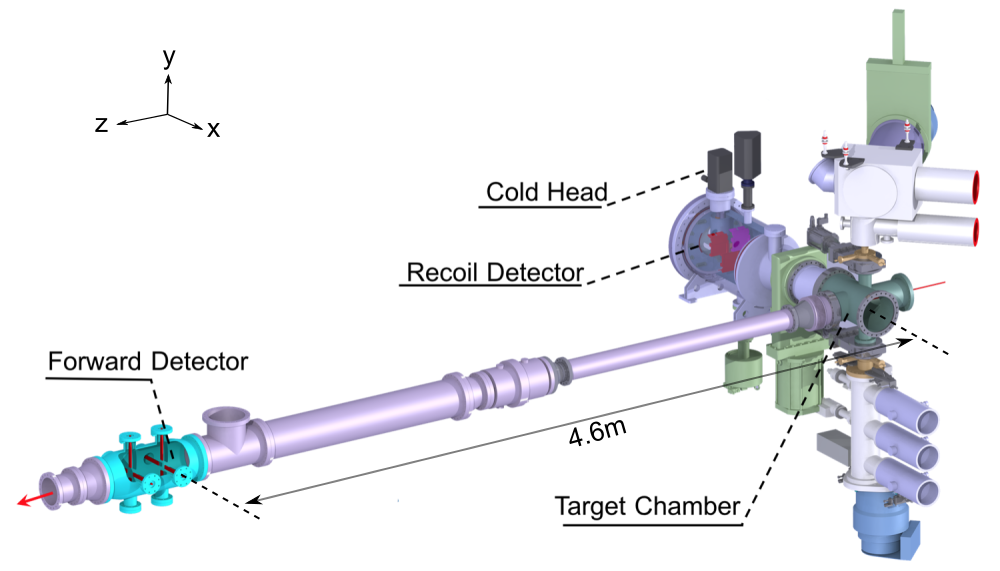
\includegraphics[width=0.8\textwidth]{./koala_setup.png}
	\caption{3D visualization of KOALA setup at COSY}
	\label{fig:setup}
\end{figure*}

The KOALA experiment is a fixed-target experiment aiming to measure the
differential cross-section of $\bar{p}p$ or $pp$ elastic scattering
over the four-momentum transfer range $0.0008 < |t| < \SI{0.1}{\tmom}$, which
covers the CNI region.
Due to the identical kinematics of $\bar{p}p$ and $pp$ elastic scattering, the
same setup of KOALA can be used in both measurements.
It is scheduled to measure $\bar{p}p$ elastic
scattering at the future HESR ring of FAIR \cite{FAIR} in the beam momentum range from
\SIrange{1.5}{15}{\momentum}.
Before the commission of HESR, KOALA is scheduled to be ran at COSY \cite{COSY}
for measuring $pp$ elastic scattering in the beam momentum range from \SIrange{1.5}{3.4}{\momentum}.
Over these beam energy range, KOALA covers the different regions where the Coulomb interaction, the CNI and the nuclear interaction are all significant.
The so called Coulomb normalization method \cite{bernard1987real,jenni2008atlas} can be used once Coulomb region is reached.
This enables the possibility of the determination of \({\sigma}_{tot}\), \(b\), \(\rho\) as well as
the absolute luminosity by analyzing the characteristic shape of $dN/dt$
spectrum (i.e. relative differential cross section) \cite{recoil_article}.
The absolute differential cross section can be normalized accordingly.

Due to the limitation of beam pipe aperture and the beam emittance,
it is extremely difficult to measure the scattering particle over a wide range of scattering angle in the forward direction.
The recoil measurement technique ,which means precise measurement of both the recoil angle and the kinetic energy of the recoil proton, 
is used to determine the differential elastic scattering cross section in KOALA.
Identification of the elastic scattering events is based on the match between the recoil angle and the kinetic energy.
A recoil detector based on this idea has already been built and the method of recoil measurement technique was verified using proton beams at COSY \cite{recoil_article}.
It was found in these tests that the identification of elastic events was limited by the large contamination of low-energy
background events at very small recoil angles, which correspond to $|t| <
\SI{0.001}{\tmom}$.
These backgrounds are mainly from inelastic scattering processes.

% To reach the remaining range \(0.0008 < |t| < 0.001\) \((GeV/c)^2\) in KOALA, a coincidence measurement between the recoil proton and scattering beam particle is proposed to suppress the background contamination.
% A time-sensing forward detector with a limited coverage range at small scattering angle is designed and built for this purpose. 
% the coincidence measurement between the recoil proton and scattering beam particle is proposed.
In order to suppress these backgrounds and achieve the designed t-range of the
differential cross section, a forward detector based on fast-timing plastic scintillator is
employed to measure the elastically scattered beam particle near the beam axis.
This full setup of KOALA , consisting of the recoil detector, the newly-built forward detector and other upgraded components,  are installed at COSY.
Several tests using proton beams have been carried out to verify the design and the performance.
In the following sections,  the full system of KOALA at COSY is described and the preliminary results from the beam tests are presented.

\section{Experimental setup at COSY}
\label{sec:setup}

KOALA is installed at a linear section in the COSY ring.
The setup consists of three arms as shown in Fig. \ref{fig:setup}: the hydrogen
cluster target arm, the recoil arm and the forward arm.
All components inside these arms are installed in the same vacuum space as the beam.

The hydrogen cluster target connects vertically to the target chamber, with the target generator on the top and the target beam dump on the bottom.
The recoil arm is oriented along -X axis of the laboratory frame.
The chamber holding the recoil detector sensors are separated with target
chamber with a vacuum gate valve.
This valve is used for staged pumping of the recoil chamber during the
preparation of the experiment and protects the recoil sensors from the residual
gas inside the beam pipe.
The forward chamber locates about \SI{4.6}{\meter} away from the target center and
connects to the target chamber through two beam pipes with the diameter \SI{90}{\mm} and \SI{200}{\mm} respectively. 

\subsection{Hydrogen cluster target}
\label{sec:target}

A thin hydrogen cluster target, which can be operated under ultra high vacuum
environment, is critical for the sucess of KOALA.
First, the energy loss of recoil proton before hitting the recoil sensor should
be minimized so that an accurate determination of its kinetic energy is possible.
Second, the thickness of the target (i.e. the profile along the beam direction) determines
the spread of the vertex distribution of beam-target interaction.
Since there is no tracking device in KOALA, the spread will deteriorate the
angular resolution as well as the energy spectrum shape.

The hydrogen cluster target, which was used previously in ANKE experiment
\cite{cluster_target}, is upgraded in KOALA.
A special collimator is built to achieve a much
smaller width of the cluster along the beam axis.
The target thickness is measured to be $\sim\SI{2}{\mm}$ in the target chamber center.
The areal density is estimated to be \SI{e14}{\atom\per\cm\squared}.

\subsection{Recoil detector}
\label{sec:recoil}

The recoil detector needs to totally stop the recoil proton from the
elastic scattering and measure its total kinetic energy.
For elastic scattering of two particles with the same mass,
the kinetic energy of recoil proton \(T_p\) is proportional to four-momentum
transfer squared by \(|t| = 2m_pT_p\), where \(m_p\) is the proton mass.
For the maximum $|t|=\SI{0.1}{\tmom}$, \(T_p \approx \SI{54}{\MeV}\). Thus, a dynamic range of
$0\sim\SI{60}{\MeV}$ is required of the recoil detector.

\begin{figure}[htbp]
  \centering
  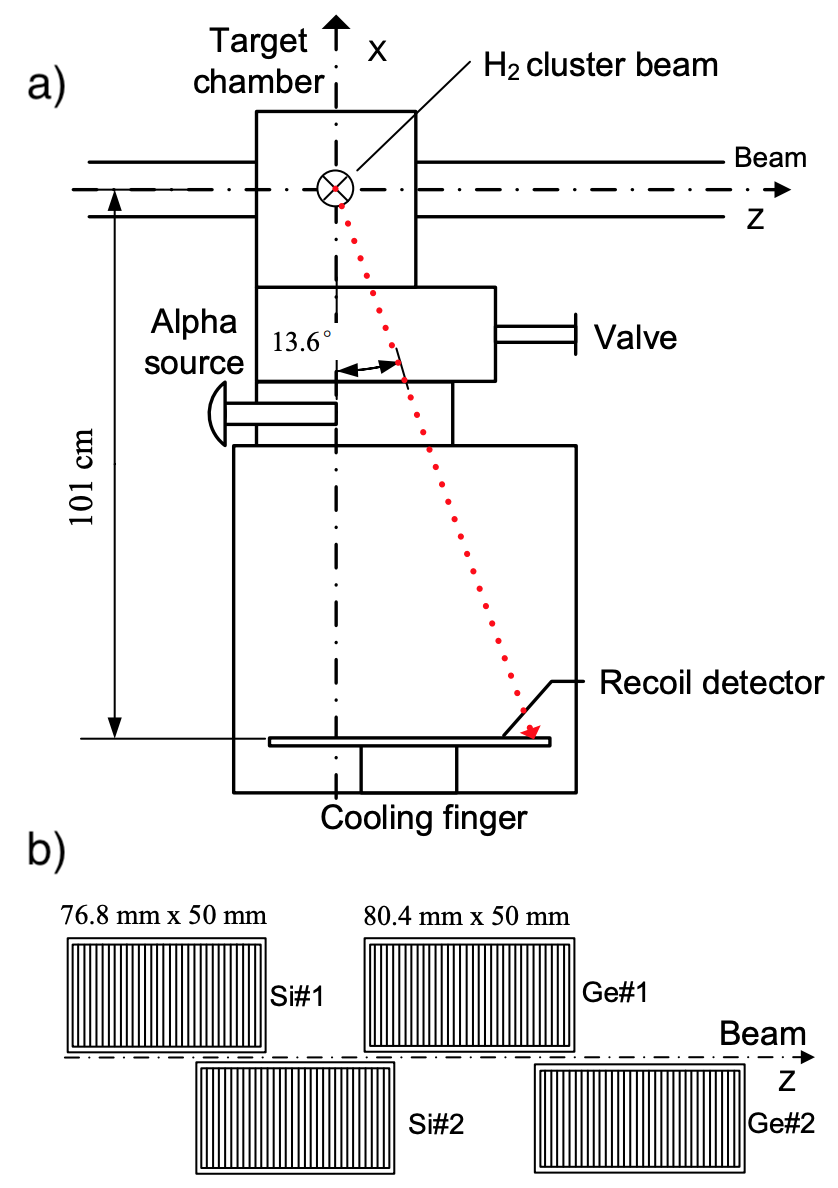
\includegraphics[width=0.4\textwidth]{./recoil_schematic.png}
  \caption{(a) Schematic view of the recoil detector configuration, seen from the
    top; (b) Layout of the four recoil sensors, seen from +X direction}
  \label{fig:recoil_schematic}
\end{figure}

The recoil detector consists of two single-sided silicon strip sensors and two
single-sided germanium strip sensors with a layout shown in Fig. \ref{fig:recoil_schematic}.
The detector plane is installed \SI{90.4}{\cm} away from the beam-target center
and covers a range of recoil angle $\SI{-1.5}{\degree} < \alpha < \SI{15}{\degree}$.
The sensors are arranged along the beam axis with staggered placement in the Y-axis.
Sensors at different recoil angle have different thickness: \SI{1}{\mm} for Si1
and Si2, \SI{5}{\mm} for Ge1 and \SI{11}{\mm} for Ge2.
The silicon sensors have an sensitive area of $76.8 \times \SI{50}{\mm\squared}$, which are
segmented into 64 strips of \SI{1.2}{\mm} pitch.
The germanium sensors have an sensitive area of \(80.4 \times \SI{50}{\mm\squared}\), which are segmented into 67 strips of \SI{1.2}{\mm} pitch.
This gives an angular resolution of about \SI{0.08}{\degree}.
By design, neighboring sensors have an overlapping region which is symmetric against
the beam axis (20 strips for Si1/Si2 overlapping, 9 strips for Si2/Ge1 overlapping, 10 strips for Ge1/Ge2 overlapping).
The overlapping strips are used for the sensor alignment and the correction of beam position asymmetry.

The sensors are read out by a combination of the charge-sensitive preamplifier (MPR16 for the strips, MPR1 for the rear side) 
and the timing filter amplifier (MSCF16), all from Mesytec \cite{mesytec}. 
MSCF16 integrates the shaping amplifier and the leading edge discriminator in the same module.
Both amplitude and timing signal are extracted from MSCF16 for energy and time measurement.
Strips at small recoil angle are read out by a single channel without sacrificing the angular resolution.
In total, there are 180 readout channels for the recoil detector: 
48 channels on Si1, 64 channels on Si2, 32 channels for Ge1 and Ge2 and 4
channels for the rear sides. 

Soild-state sensors (especially germanium) need low and stable operating temperature to optimize energy
resolution.
Temperature of the recoil sensors are monitored by four temperature sensors
attached to the detector holder.
The operating temperature can be actively adjusted by a combination of a cold head and two heating resistors on the cold plate.
A study of the performance of recoil sensors in the laboratory shows that the
optimal working temperature of the recoil detector is \SI{125}{\kelvin}.
Under this condition, the energy resolutions of the silicon and germanium
sensors are better than \SI{20}{\keV} and \SI{30}{\keV} (FWHM) respectively.

More technical information and the detailed performance tests of the recoil detector can be found in \cite{recoil_article}.

\subsection{Forward detector}
\label{sec:fwd}

The forward detector aims to detect the elastically scattered beam proton in the
forward direction and measure its arrival time.

As shown in Fig. \ref{fig:setup}, it consists of 8 detector modules, which are grouped into 2 layers and 4 pairs.
The 4 pairs are installed symmetrically on +X, -X, +Y and -Y axis, with the same
distance of \SI{3}{\mm} away from the beam pipe center.
The first layer of each pair are installed \SI{4.6}{\meter} away from the
beam-target center, and the seperation between the two layer is \SI{20}{\cm}.
Only the pair on -X is used for the conincidence measurement with the recoil detector.
The other 3 pairs are used for beam position tuning during beam preparation and
monitoring during the experiment.

Each detector module is made of plastic scintillator BC-408 \cite{bc408} with the dimension $90 (length) \times 20 (width) \times 6
(thickness)\,\si{\mm\tothe{3}}$.
% This corresponds to an angular acceptance of $\SI{0.37}{\degree} < \theta < \SI{1.49}{\degree}$.
The length of the scintillator guarantees the required coverage
from \SI{0.0008}{\tmom} to \SI{0.001}{\tmom} longitudinally over the COSY energy range.
However, the cross-sectional coverage, \textit{i.e.}, the coverage of the full length of
the recoil detector strips, depends not only on the beam energy but also on the
size of beam profile.
Fig. \ref{fig:forward_acceptance} shows an example of the impact of beam emittance on the
effective cross-sectional coverage.
The fully-covered area on the recoil detector shrinks with the increasing of beam emittance. 
\begin{figure}[htbp]
  \centering
  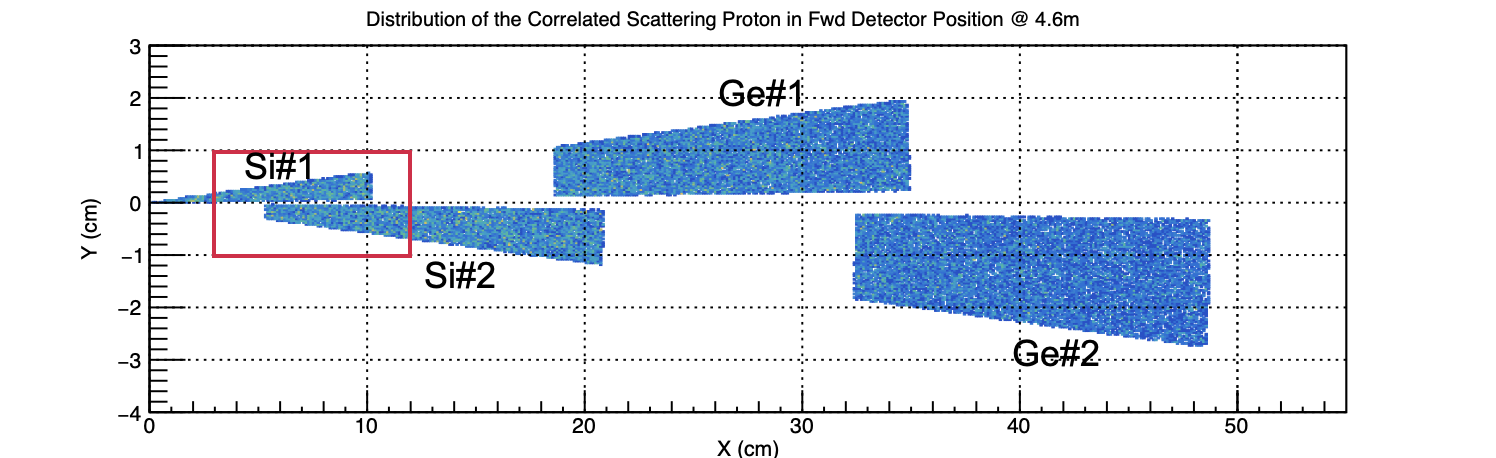
\includegraphics[width=0.45\textwidth]{./fwd_acceptance.png}
  \caption{
    Hit position distribution of the elastically scattered proton on the X-Y plane at \SI{4.6}{\meter}
    from the beam-target center. The results are from the simulation of \SI{2.2}{\momentum}
    $pp$ elasitc scattering with an uniform spherical distribution in the
    center-of-mass reference frame: up) ideal point beam; down) $\SI{10}{\mm}\times\SI{10}{\mm}$ box beam profile.
    % for the elastic scattering events in which
    % the recoil proton hits one of the recoil sensors.
    The four blue blocks are from the events in which the recoil proton hits one of
    the four recoil sensors.
    The red square indicates the dimension of the forward detector scintillator
    and the vertical dashed line indicates the hit position when $|t| = \SI{0.001}{\tmom}$.}
  \label{fig:forward_acceptance}
\end{figure}
Based simulation study, the current width of the forward detector scintillator guarantees the
full cross-sectional coverage for $|t| < \SI{0.001}{\tmom}$ as long as the beam profile size is smaller than \SI{7}{\mm}.

The scintillator is readout by the combination of a tapered light guide, a piece of silicone pad and a
photomultiplier tube (Hamamastu H6900 \cite{hamamatsu}), as shown in Fig. \ref{fig:forward_module} (a).
Each detector module is integrated with a forward chamber flange for the usage
in the ultra-high vacuum environment.
To protect the vacuum condition inside the beam pipe, the following designs are implemented:
\begin{enumerate}
\item only the light guide and the scintillator are installed inside the forward chamber, the light guide is glued on the open port of the flange as a feedthrough;
\item no wrapping and painting material on the surface of the scintillator, the surface is polished to increase light collection efficiency;
\item a thin aluminum tube with thickness of \SI{100}{\micro\meter} is used as
  the light shield of the scintillator, the tube is screwed on the flange, see Fig. \ref{fig:forward_module} (b);
\item two small holes are opened on the side of the aluminum tube to speed up vacuum pumping, see Fig. \ref{fig:forward_module} (c).
\end{enumerate}
Other components like the silicone pad, the PMT and the PMT base are installed inside a light-tight case on the other side of the flange as shown in Fig. \ref{fig:forward_module} (c).
\begin{figure}[htbp]
  \centering
  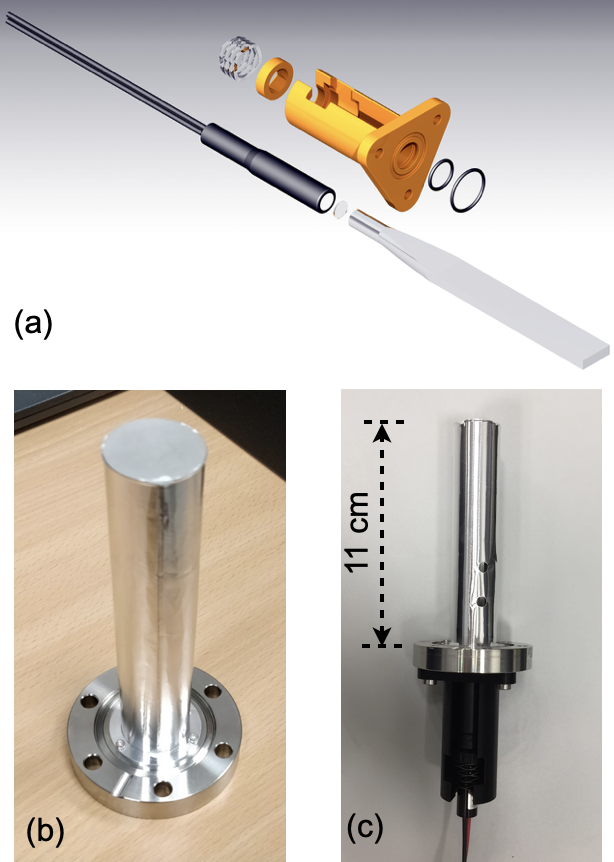
\includegraphics[width=0.32\textwidth]{./forward_module.png}
  \caption{(a) CAD model of the assembly of forward detector module; (b) The aluminum tube is fixed on the inside of the flange; (c) One forward detector module after complete assembly}
  \label{fig:forward_module}
\end{figure}
% \begin{figure}[htbp]
%   \centering
%   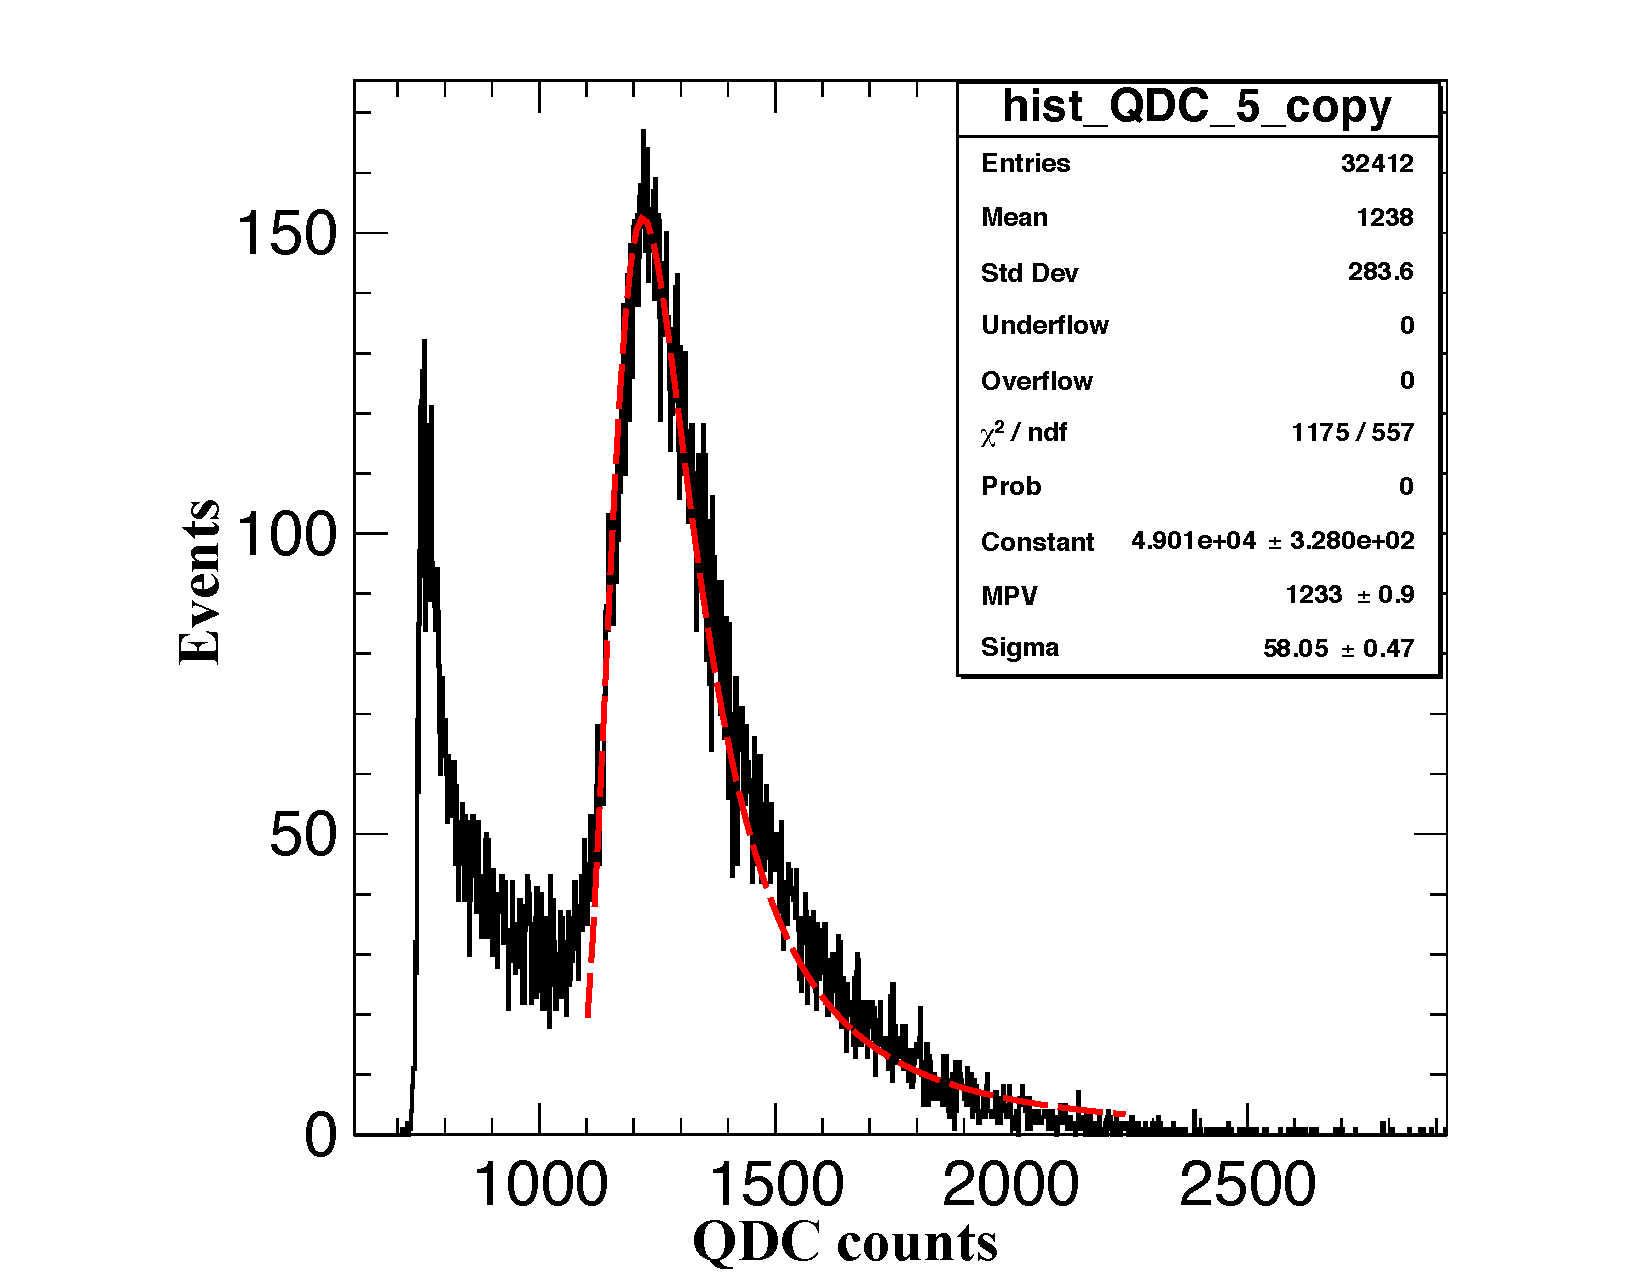
\includegraphics[width=0.4\textwidth]{./forward_mip.pdf}
%   \caption{An example of the cosmic ray energy spectrum obtained by a forward detector module}
%   \label{fig:forward_mip}
% \end{figure}

Due to the large gain of PMT, no front-end electronics is needed for the readout of the forward detector.
The output signal from H6900 is split into two branches: one fed to a
constant fraction discriminator for time information extraction; the other for charge measurement directly.
Modules are tested using cosmic ray in laboratory before installation.
% A typical MIP spectrum obtained by the forward detector module is shown in Fig. \ref{fig:forward_mip}. 
The peak of minimum ionizing particle (MIP) is well separated from the pedestal noise, with signal to noise ratio larger than 50.
The timing resolution is measured to be about \SI{140}{\pico\second}.

\begin{figure*}[htbp]
  \centering
  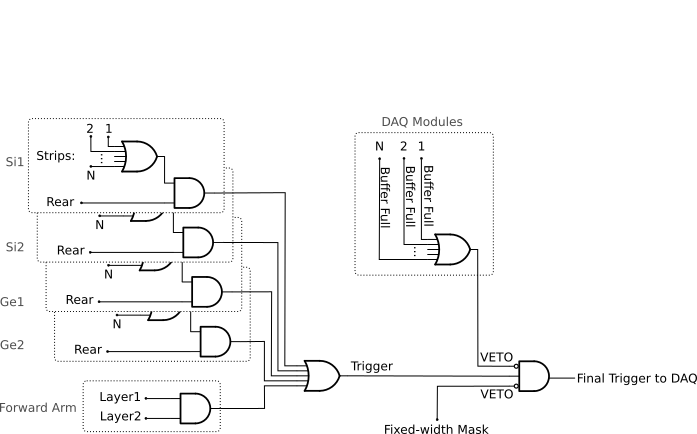
\includegraphics[width=0.75\textwidth]{./trigger_logic.png}
  \caption{Trigger Logic of the KOALA DAQ.}
  \label{fig:trigger_logic}
\end{figure*}

\section{Data acquisition system}
\label{sec:daq}

The data acquisition system of KOALA is a VME-based system with multiple types
of digitization modules produced by Mesytec \cite{mesytec}.
For the recoil detector, the amplitude signal from MSCF16 is digitized by a
peak-sensing ADC module MADC-32.
MADC-32 has a 13-bit dynamic range with \SI{6.4}{\micro\second} conversion time.
For the forward detector, the pulses from PMTs are directly fed into a QDC
module MQDC-32 for the charge measurement.
MQDC-32 has a dynamic range of \SI{500}{\pico\coulomb} with 12-bit resolution
and \SI{250}{\nano\second} conversion time.
The timing information from both the recoil and forward detectors are recorded by a TDC module MTDC-32 using the conventional Start-Stop method.
MTDC-32 has a minimum resolution of \SI{5}{\pico\second}.
A multi-channel scalar SIS3820 \cite{sis} is also integrated to record
the following key count rates: 1) count rates of the four pairs of the forward detector for beam position monitoring; 2) count rates of the overlapping regions of the recoil detector for asymmetry correction; 3) count rates of the input trigger
for DAQ efficiency correction.

% The acceptance of the forward detector only covers a small part of the recoil detector sensors.
% To record the elastic scattering events from the whole range of the recoil angle
% covered by the recoil detector,
KOALA adopts a self-triggering scheme for the trigger logic design.
Each sensor of the recoil detector and each arm of the forward detector works independently and generates their own trigger. 
The final trigger to the DAQ is a common OR of all sub-detectors, as shown in Fig. \ref{fig:trigger_logic}.
The trigger from the recoil detector sensor is generated by a coincidence between the front-side strips and the rear-side plane, 
and the trigger from the forward detector arm is generated by a coincidence between the two modules in the same pair.
% In this way, the rate of the false hits generated by electronic noise can be minimized.
Both elastic and inelastic scattering events are recorded in this trigger design, and the coincidence between the recoil sensor and the forward detector is carried out in offline analysis.

Fast readout of the recorded event is crucial for a self-triggered DAQ system.
The asynchronous readout mechanism combined with VME CBLT block read mode is adopted to increase the data throughput in KOALA.
The digitization modules used in KOALA all have an event buffer with a size
larger than \SI{32}{\kilo\byte}.
Digitized events are stored in this buffer before readout, so that the module is immediately available to digitize the next event.
Events will not be readout until the buffer is nearly full.
Since the cross section is higher at smaller recoil angle, the module for these channels always saturates faster than others.
Modules with a saturated event buffer may miss new coming events while others
not, and thus bringing a systematic bias.
To overcome this issue, the buffer-full signal from each module is added to the trigger logic as \texttt{VETO} as shown in Fig. \ref{fig:trigger_logic}.

The issue about event synchronization arises naturally when using asynchronous
readout mode.
% The digitization modules used in KOALA have different dead time, especially between MADC-32 and MTDC-32.
% An event recorded by a fast module may be missed by a slow module. This creates un-synchronous event structure, which makes the sequential event data assembling impossible. 
Timestamp-based synchronization is used to solve this problem.
The modules in the system have a 30-bit counter for recording the timestamp from
the clock signal distributed by a central source.
The source could be either the VME built-in clock (\SI{16}{\MHz}) or an external clock
(lower than \SI{75}{\MHz}).
Currently, the built-in clock of VME backplane bus is used. 
Based on this timestamp, event synchronization is achieved offline.
The other option is adding a fixed-width mask gate into the trigger logic as \texttt{VETO}, see Fig. \ref{fig:trigger_logic}.
The width of the mask gate should be larger than the maximum dead time of all modules.
In this way, the events are effectively synchronized sequentially. 
However, this method may reduce DAQ efficiency significantly in a high hit-rate environment.

\begin{figure}[htbp]
\centering
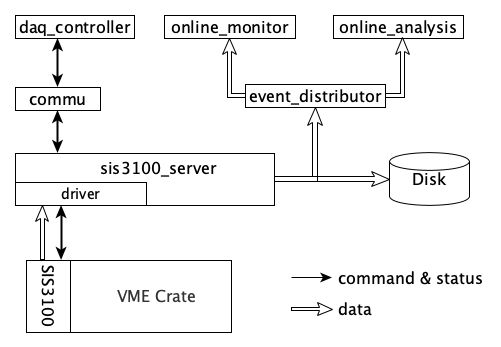
\includegraphics[width=0.45\textwidth]{./koalaems_deployment.png}
\caption{Design and deployment of KoalaEms.}
\label{fig:koalaems}
\end{figure}

% \raggedright
A dedicated DAQ software called KoalaEms is also developed for KOALA.
KoalaEms is a fork of the EMS software \cite{ems}, which is a highly flexible DAQ software framework developed for various experiments at COSY.
Support for the VME controller (SIS3100 \cite{sis}) is integrated and a new component of online monitoring based on ROOT is added.
The architecture of KoalaEms is shown in Fig. \ref{fig:koalaems}.
The interface to the DAQ is implemented as \linebreak\texttt{sis3100\textunderscore server}, the host of which
connects to SIS3100 by an optical link.
The control and status information from/to the GUI \texttt{daq\textunderscore controller} is mediated by a component called \texttt{commu}.
The data flow from VME crate is split into two branches: 1) \texttt{data\textunderscore out\textunderscore disk}: save the raw data onto disk; 2) \texttt{data\textunderscore out\textunderscore stream}: stream out to \texttt{event\textunderscore distributor}.
\texttt{event\textunderscore distributor} will forward the data stream to various consumption hosts for usages like online monitoring and online analysis.
Both \texttt{commu} and \texttt{event\textunderscore distributor} support socket connection and the \texttt{event\textunderscore distributor} also supports multiplexing streaming.
All the square blocks in Fig. \ref{fig:koalaems} can be hosted in different PC and new consumption host to the data stream can be integrated whenever needed.
% \justify

\section{Software framework}
\label{sec:software}

A dedicated software framework called KoalaSoft is developped for the simulation, calibration, reconstruction and analysis jobs of the KOALA experiment.
It is built upon the FairRoot \cite{fairroot} framework, which implements a simulation environment based on VMC \cite{vmc} library and an analysis environment based on ROOT's task concept.
The components stack of KoalaSoft is shown in Fig. \ref{fig:koalasoft}.

\begin{figure}[htbp]
  \centering
  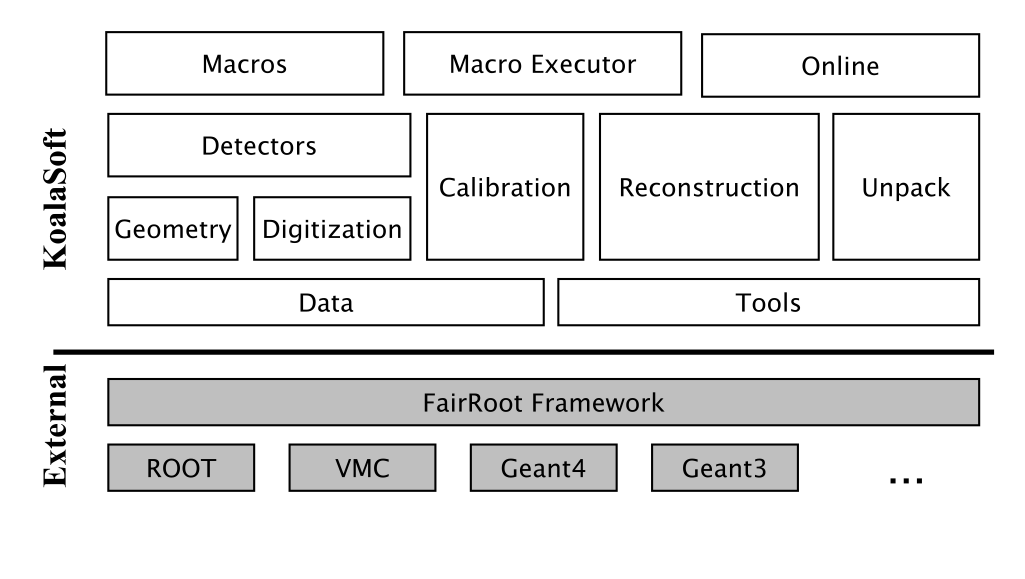
\includegraphics[width=0.48\textwidth]{./koalasoft_components.png}
  \caption{Components of KoalaSoft}
  \label{fig:koalasoft}
\end{figure}

Both Geant3 and Geant4 can be selected as the simulation engine without changing other components in KoalaSoft.
Geometry models of the recoil detector and the forward detector are implemented using ROOT's TGeo library.
Jobs like digitization, calibration and reconstruction are divided into multiple smaller steps, each of which is represented by a single task.
Tasks chained together later in a ROOT macro to compose a full job. 
ROOT macros are the interface for the end user using KoalaSoft.
Macros for common jobs are pre-configured and distributed along with KoalaSoft.
Users can also compose their own specific jobs for analysis.
Additionally, a binary macro executor is provided to run jobs directly from command line. This may be useful in batch processing.

In KoalaSoft, the same chain of tasks can be used for the analysis of both the simulation data and the raw data from DAQ.
This is accomplished by the \texttt{Unpack} component, which can decode and transform the raw binary data into the same format as the output from simulation jobs.
Algorithms developped, tested and verified using simulation data can be applied to experimental data seamlessly.
This saves a lot of efforts in the development and maintainence of algorithms.
Both the offline disk data and the online streaming data are correctly handled by \texttt{Unpack} and an online monitoring program is developped based on it.

\section{Reconstruction}
\label{sec:reconstruction}

\subsection{Energy calibration}
\label{sec:calibration}

\begin{figure*}[htbp]
\centering
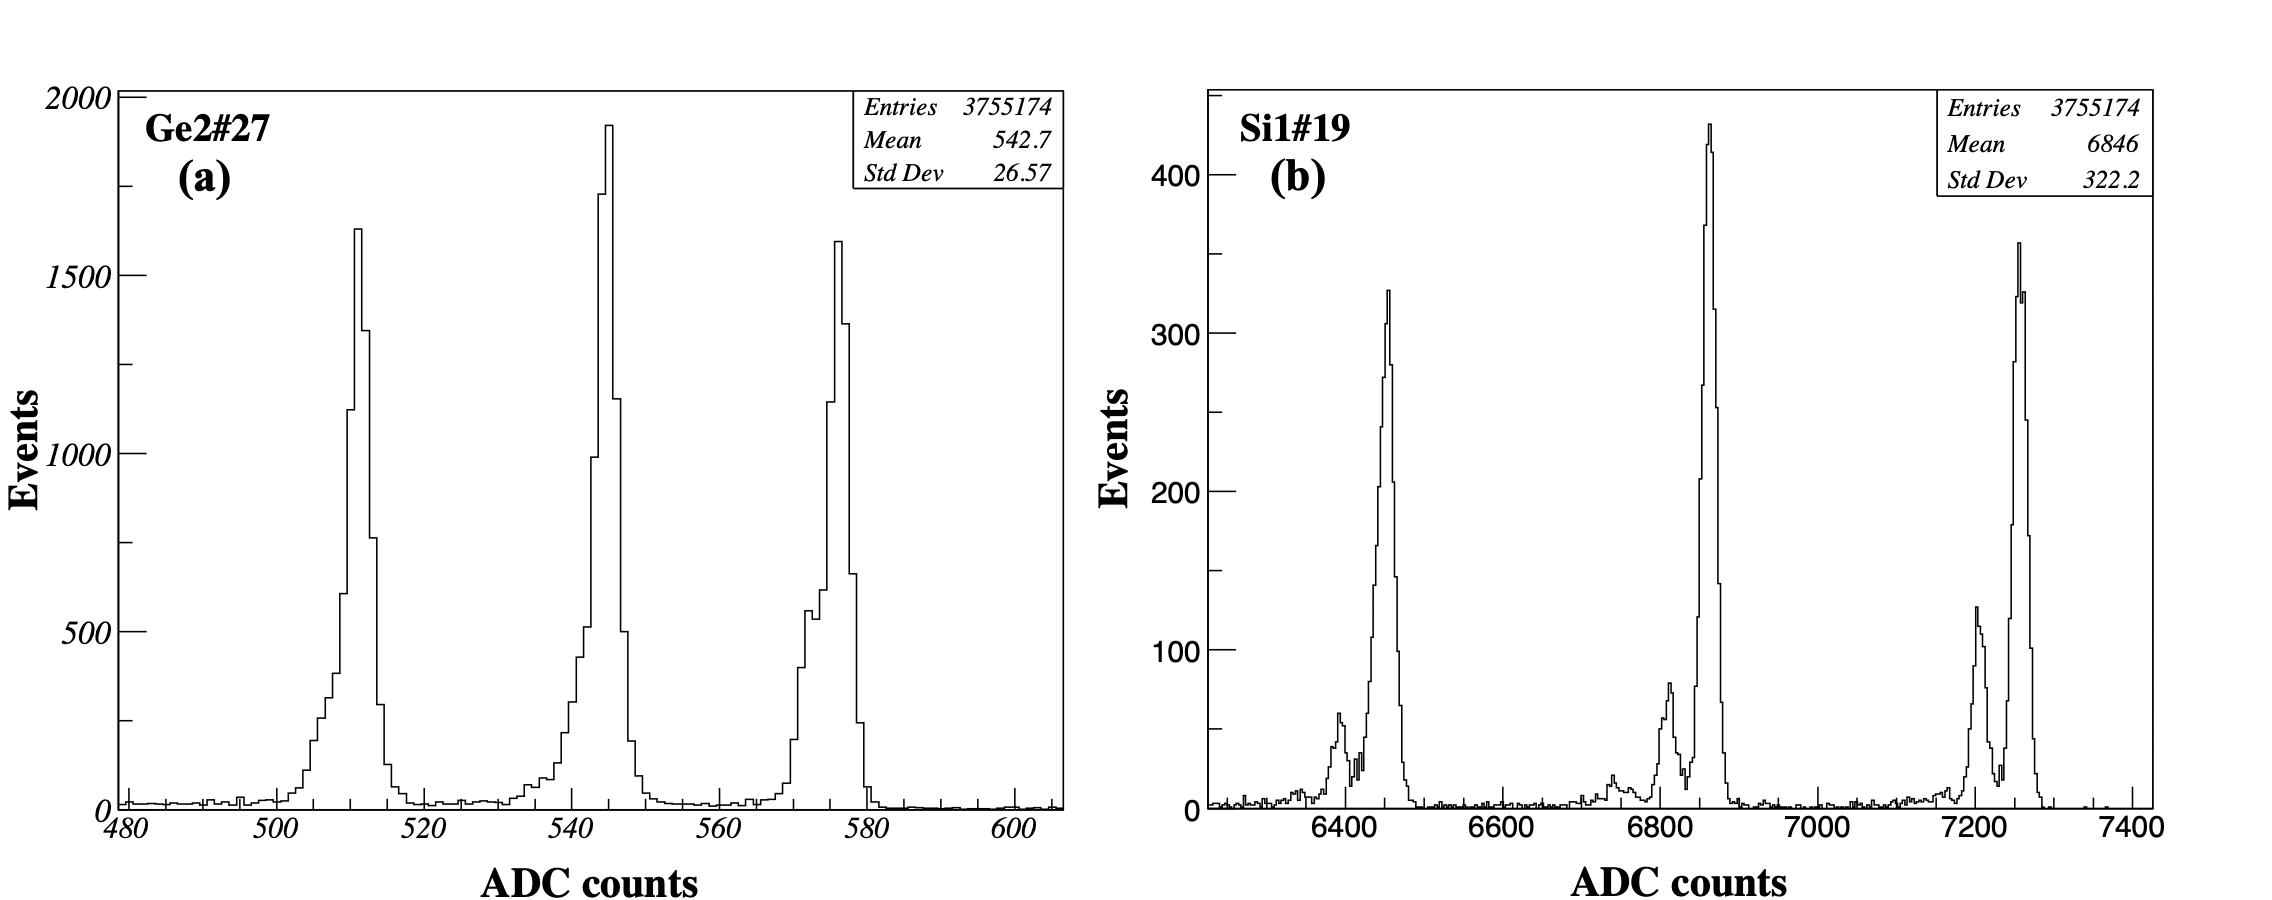
\includegraphics[width=0.8\textwidth]{./alpha_response.png}
\caption{Example energy spectrums of \(\alpha\) sources of two channels at different positions: (a) large recoil angle $13.9\degree$; (b) small recoil angle $0.93\degree$}
\label{fig:alpha_spectrum}
\end{figure*}

% Precise measurement of energy deposit in the recoil detector is critical for the
% identification of elastic scattering events as well as the calculation of the recoil angle.
\(\alpha\) sources \(^{239}Pu\), \(^{244}Cm\), \(^{241}Am\), with decay energies of \SIlist{5156.59;5804.83;5485.56}{\keV} \cite{nuclear_data} respectively, are used for the energy calibration.
Decays with much smaller branch ratios also exist in these sources. They may also be used in the energy calibration if they are well separated from the main peaks.
$\alpha$ sources are installed inside the recoil chamber and fixed on a linear motion feedthrough rod.
During experiment, the rod is lifted and the sources are blocked by the chamber wall;
when calibration is needed, the rod is pushed to the chamber center and the sources face the recoil sensors directly.
Thus, the recoil detector can be calibrated regularly when no beam is circulating.

Two aspects need special consideration in the calibration.
First, the recoil sensors have a protective layer on the surface. 
\(\alpha\) particles will lose some energy in this layer before entering the
fiducial volume of the sensor.
The thickness of the protection layer has been measured in the laboratory using \(\gamma\) rays \cite{recoil_article}.
The energy loss in the protection layer is calculated and shown in Tab. \ref{tab:dead_layer} for each $\alpha$ energy when the incidence angle is \SI{90}{\degree}.
The effective energy deposit in the fiducial volume is further corrected based
on the recoil angle of each strip.

\begin{table}[htbp]
\label{tab:dead_layer}
\caption{Energy loss (keV) of $\alpha$ in the protection layer when incidence angle is \SI{90}{\degree}}
\centering
\begin{tabular}{cccccc}
\hline
\(E_{\alpha} (keV)\) & \(\Delta E_{Si1}\) & \(\Delta E_{Si2}\) & \(\Delta E_{Ge1}\) & \(\Delta E_{Ge2}\) \\
\hline
5156.59 & 11.51 & 11.51 & 110.00 & 111.00 \\
5485.56 & 11.01 & 11.01 & 105.00 & 106.00 \\
5804.83 & 10.52 & 10.52 & 99.00  & 100.00 \\
\hline
\end{tabular}
\end{table}

Secondly, the gain setting of each readout channel is optimized for the recoil
energy range covered by the strip.
The gain difference can vary up to a factor of about 10.
Thus, the resolution is worse at large recoil angle than at small angle, as shown in Fig. \ref{fig:alpha_spectrum}.
The minor decay modes can't be recognized in Fig. \ref{fig:alpha_spectrum} (a), while they are clearly seen in Fig. \ref{fig:alpha_spectrum} (b).
Since only three energy points can be used, lower resolution brings larger systematic error in the calibration.

\begin{figure}[htbp]
\centering
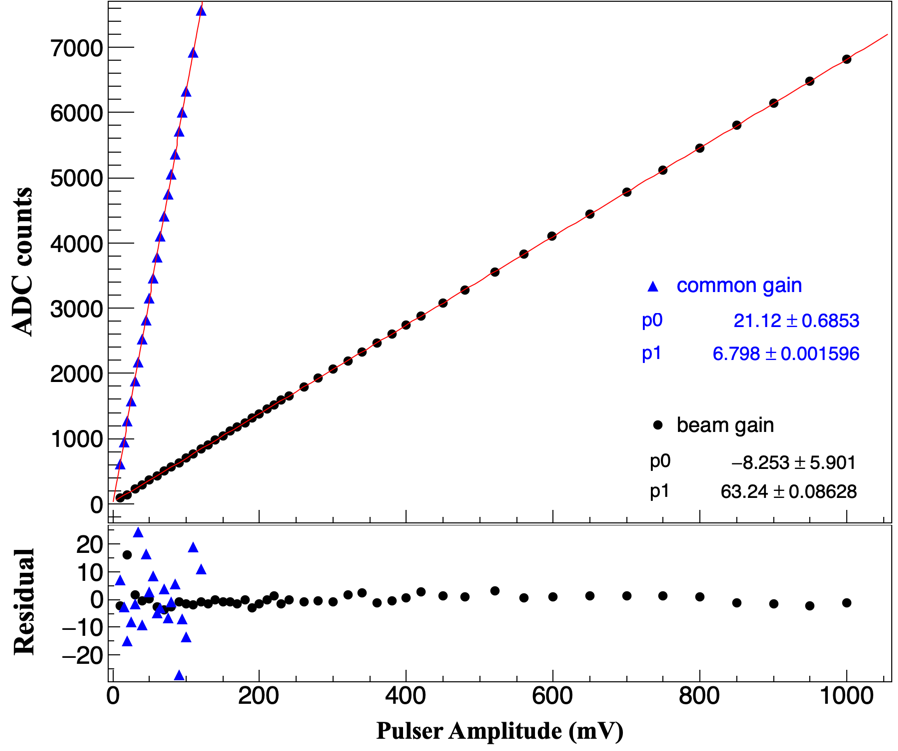
\includegraphics[width=0.42\textwidth]{./linearity.png}
\caption{Electronic linearity of a typical recoil detector channel}
\label{fig:electronic_linearity}
\end{figure}

To minimize this error, a common gain, which is optimized for the separation of the \(\alpha\) energy peaks, is set for all channels.
The calibration is carried out as follows:
\begin{enumerate}
\item the energy spectrum of the \(\alpha\) sources is recorded under the common gain setting and the energy peaks are searched;
\item the gain difference between the common gain and the beam gain setting used
  in experiment is measured by scanning a precision analog pulser over a large range of amplitudes;
\item the energy responses at beam gain setting are then deduced by applying the gain
  difference to the common gain responses, and the result is fitted using a linear function.
\end{enumerate}
The fitting parameters of the last step are the parameters used to convert ADC
values into energy in the reconstruction.
% The readout electronics of the recoil detector has very good linearity in both
% common gain and beam gain setting (see Fig. \ref{fig:electronic_linearity}), thus no extra systematic bias is brought in.
Due to the good linearity of the readout electronics in both common gain
and beam gain setting (see Fig. \ref{fig:electronic_linearity}), this indirect
method does not bring in extra systematic bias.
The achieved precsion of the calibration is about \SI{0.12}{\percent}.

\subsection{Time walk correction}
\label{sec:timewalk}

Time walk effect of the leading edge discriminator used in the recoil detector needs to be corrected to
optimize the timing resoultion.
Calibration of the time-walk effect is carried out using a  precision analog pulser. 
Output of the pulser is split into two branches: one is fed into a constant fraction discriminator to generate the reference time;
the other is connected to the detector channel under calibration for measurment. 
By scanning the pulser over a wide range of amplitudes, the time-walk effect is
revealed.
An example is shown in Fig. \ref{fig:timewalk}, where the result is fitted with \(y=p_0 x^{-1} + p_1\). 
The time walk is corrected by substracting \(\Delta t = p_0/ADC\) from the
measured timing value.

\begin{figure}[htbp]
  \centering
  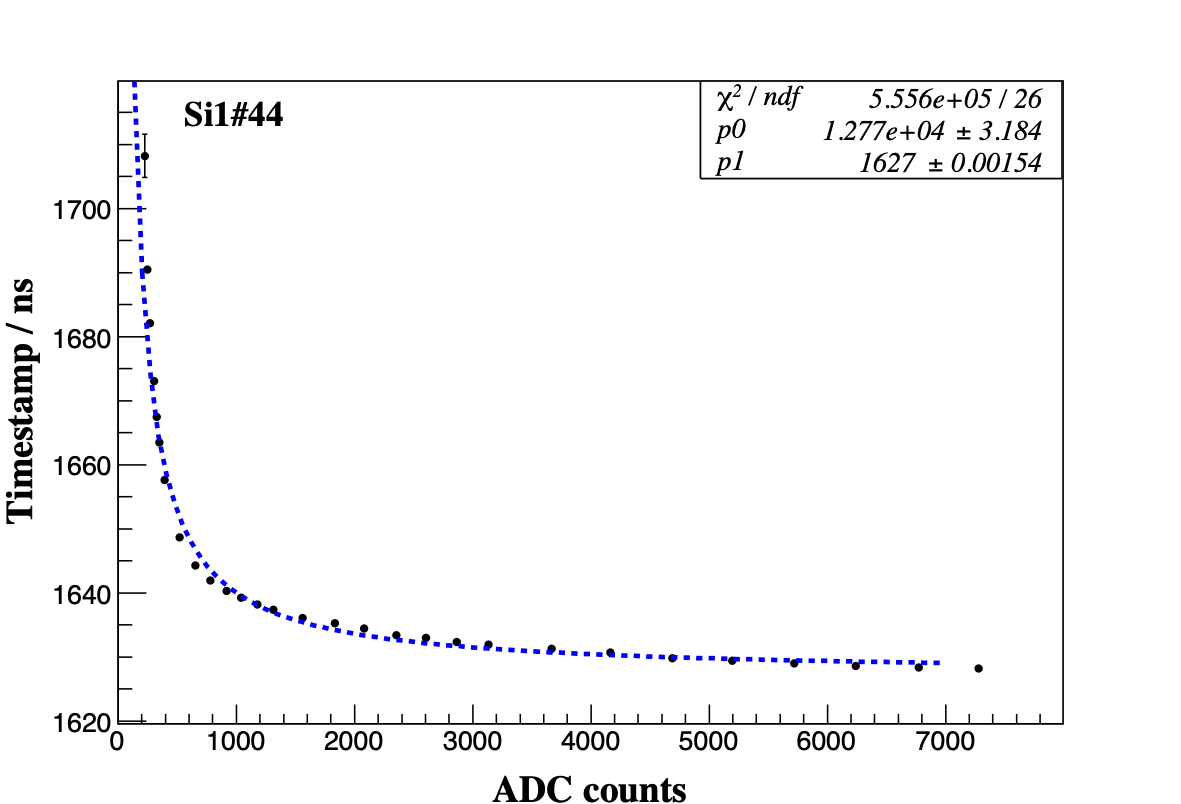
\includegraphics[width=0.45\textwidth]{./timewalk.png}
  \caption{Typical result from the time-walk calilbration.}
  \label{fig:timewalk}
\end{figure}

Moreover, the difference of the fitting paramter \(p_1\) indicates the delay time
difference between different channels, which is caused by the signal routing length variation.
These offsets are also applied in the reconstruction to align the timing from different channels.

\subsection{Clustering}
\label{clustering}

Clustering is necessary to reconstruct the correct energy deposit in the
recoil detector for the following reasons: 1) charge sharing is an intrinsic characteristic of solid-state strip detector, especially
for the tracks hitting the edge in between the adjacent strips; 2) the tracks
from beam-target interaction may penetrate through several strips before
stopping, especially for the sensors  at large recoil angle.
Both the simulation and the beam test show that about \SI{50}{\percent} of the tracks hitting Ge2 have hit multiplicity
larger than 1, see Fig. \ref{fig:multiplicity}.
\begin{figure}[htbp]
  \centering
  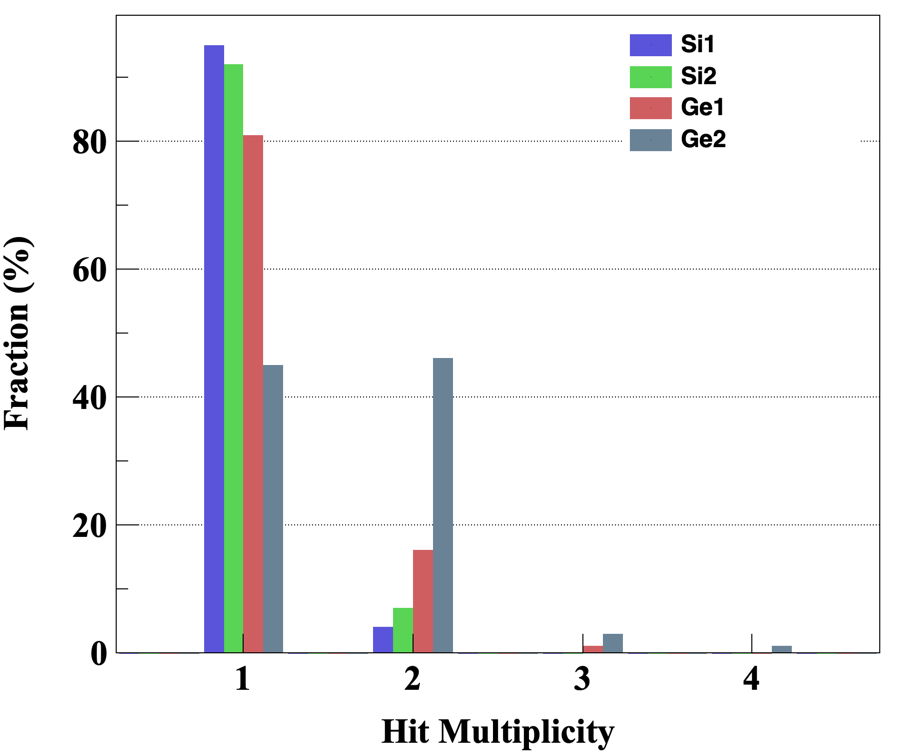
\includegraphics[width=0.45\textwidth]{./multiplicity.png}
  \caption{Fraction of the hit multiplicity on each sensor of the recoil detector.}
  \label{fig:multiplicity}
\end{figure}

\begin{table}[htbp]
  \label{tab:multiplicity}
  \caption{Hit multiplicity on the recoil detector (\si{\percent})}
  \centering
  \begin{tabular}{cccccc}
    \hline
     & 1& 2& 3&  4 \\
    \hline
    Si1 & 95.51 & 4.38 & 0.08 & 0.02 \\
    Si2 & 92.46 & 7.21 & 0.24 & 0.06 \\
    Ge1 & 81.06 & 16.61 & 1.51  & 0.44 \\
    Ge2 & 45.41 & 46.30 & 3.98  & 1.67 \\
    \hline
  \end{tabular}
\end{table}

The clustering algorithm is designed to minimize the noise contribution while
at the same time keeping the low-energy background characteristic as much as possible.
It is also important not to bring a selection bias between low energy and high energy elastic events.
The steps of clustering in KOALA is as follows:
\begin{enumerate}
\item Delete noise hits. Hits induced by the electronic noise is deleted. A low
  threshold ($2\sigma_{noise}$) is used in this step.
\item Collect remaining hits into clusters based on the adjacency principle.
\item Delete noise clusters. The noise level of cluster is evaluated as
  $\sigma_{cluster} = \sum_i^n{\sigma_{noise}^i}$, where $\sigma_{noise}^i$ is
  the noise level of each strip in the cluster. Clusters which have summed
  energy lower than $5\sigma_{cluster}$ are considered to be noise-induced and deleted.
\item Delete clusters without seed hit. Valid cluster needs to have at lease one seed hit, the
  amplitude of which exceeds the equivalent energy of the trigger threshold of
  the corresponding strip.
\end{enumerate}
The hit position and hit time of the cluster are both extracted from the first
hit in the cluster to keep the most accurate information about the recoil angle.


An example of the comparison between the energy spectrum before and after clustering is shown in
Fig. \ref{fig:clustering}.
\begin{figure}[h]
  \centering
  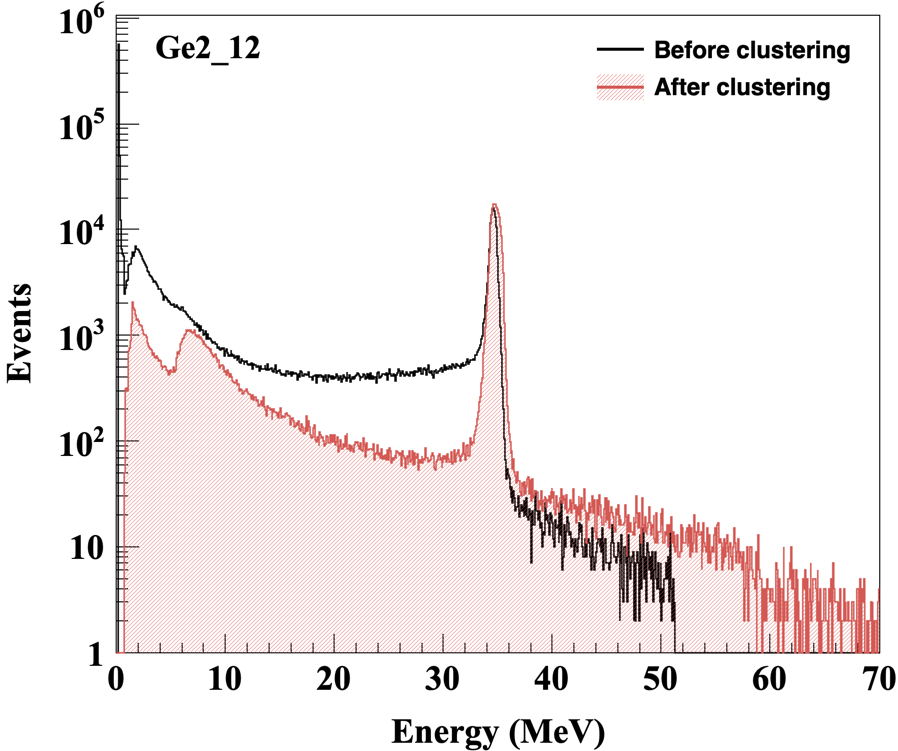
\includegraphics[width=0.45\textwidth]{./clustering.png}
  \caption{Comparison of the energy spectrum on the 12th channel of Ge2, before (black) and after
    (red) clustering.}
  \label{fig:clustering}
\end{figure}
After clustering, part of the hits on the plateau before the elastic peak, which exists in the raw spectrum before clustering, are correctly absorbed into the elastic peak.
The charasteristics of the background events also show up with two explicit
components: 1) a peak which equals MIP's energy loss in the recoil sensors; 2) a smooth decay with a long tail.
A correct modelling of the background, which is described in Sec.
\ref{sec:result}, is only possible after clustering.

\section{Beam commissioning and results}
\label{sec:result}

Beam tests were carried out using proton beam at COSY with momentum
\SIlist[list-units=single]{2.2;2.4;2.6;3.0}{\momentum} in August and October, 2019.
The analysis procedures of the beam data are the same for all momentums.
In the following, the results from \SI{2.2}{\momentum} are shown as example.

\subsection{Beam conidtion}
\label{beam}
The beam intensity of COSY is about \SI[per-mode=reciprocal]{e10}{\per\second}, with an cycle structure of
\SI{40}{\second} injection time and \SI{300}{\second} storage time, as shown in Fig. \ref{fig:beam}.
To minimize the beam emittance, stochastic beam cooling is applied in these tests.
The cooling reaches the equibilium state after the beginning $1/3$ of the storage cycle.
\begin{figure}[h]
  \centering
  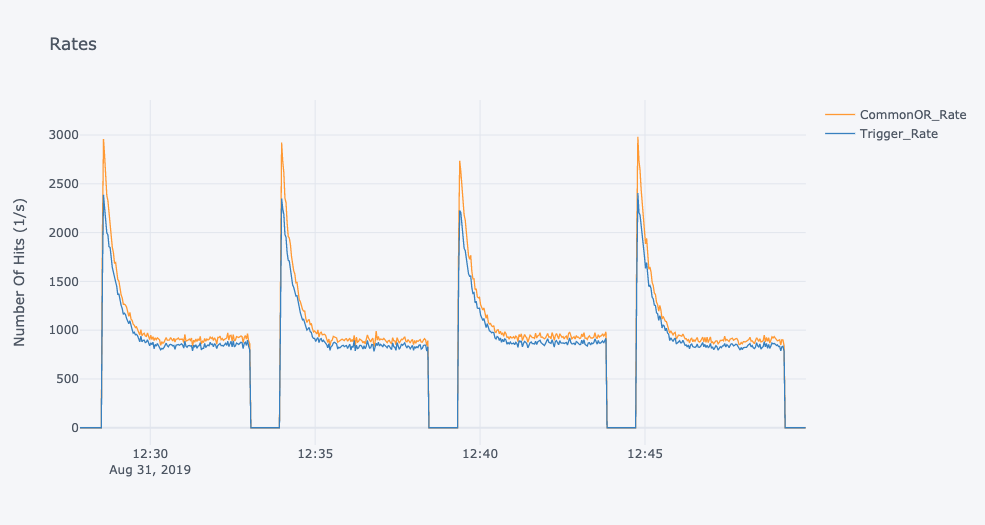
\includegraphics[width=0.45\textwidth]{./daq_efficiency.png}
  \caption{Beam cycle and DAQ efficiency.}
  \label{fig:beam}
\end{figure}
% During injection cycle, the beam has large emittance and not stable.

Only the storage cycle is used for the experiment, which is achieved by two
gates synchronized with the beam cycle.
One gate is used to protect the PMTs of the forward detector, which ramps down the high voltage supply \SI{5}{\second} before the end of the
storage cycle and ramps up the high voltage supply \SI{5}{\second} after the start of the storage cycle.
The other gate has a narrower width and is used to control the DAQ system so that data are not recorded during injection.
The DAQ efficiency in variation with the input trigger rate is also shown in Fig. \ref{fig:beam}.
A maximum of \SI{93}{\percent} is reached ,which amounts to \SI{850}{\event\per\second}.
% The efficiency is mainly limited by a wide mask gate in the trigger logic.

\subsection{Performance of the forward detector}
\label{fwd_performance}

The forward detector shows execellent performance during the beam commissioning.

By selecting the events which has at least one cluster in the recoil
detector, \textit{i.e.}, the events which triggered the recoil detector, the
characteristic responses of the two detector modules on the +X aixs are
obtained, shown as black curves in Fig.\ref {fig:fwd_performance}.
The wide peaks around \num{1200} counts on the QDC spectrum are from the beam protons
penetrating through the scintillators.
The peaks lie above a continuum background in which no distinctive thresholds can be recognized.
A further study of the response are carried out using the sample of elastic
scattering events (the selection criteria of the elastic scattering events are described in more detail in Sec. \ref{sec:elastic_extraction}).
The response of one module is obtained by using the other module for the selection.
The results are shown as the red curves in Fig. \ref{fig:performance}.
The low energy thresholds of the elastic peaks are clearly seen around \num{1000}.
They are well separated from the noise pedestals, with the signal to noise ratios about \num{40} for both detector modules.
In the analysis, these thresholds are used to select events in which the beam proton hit the forward detector.
The timing resolution (FWHM) of the forward detector is about \SI{400}{ps}, which is obtained by the dispersion of the timing difference of the two module as show in Fig. \ref{fig:performance} (c).
\begin{figure}[htb!]
  \centering
  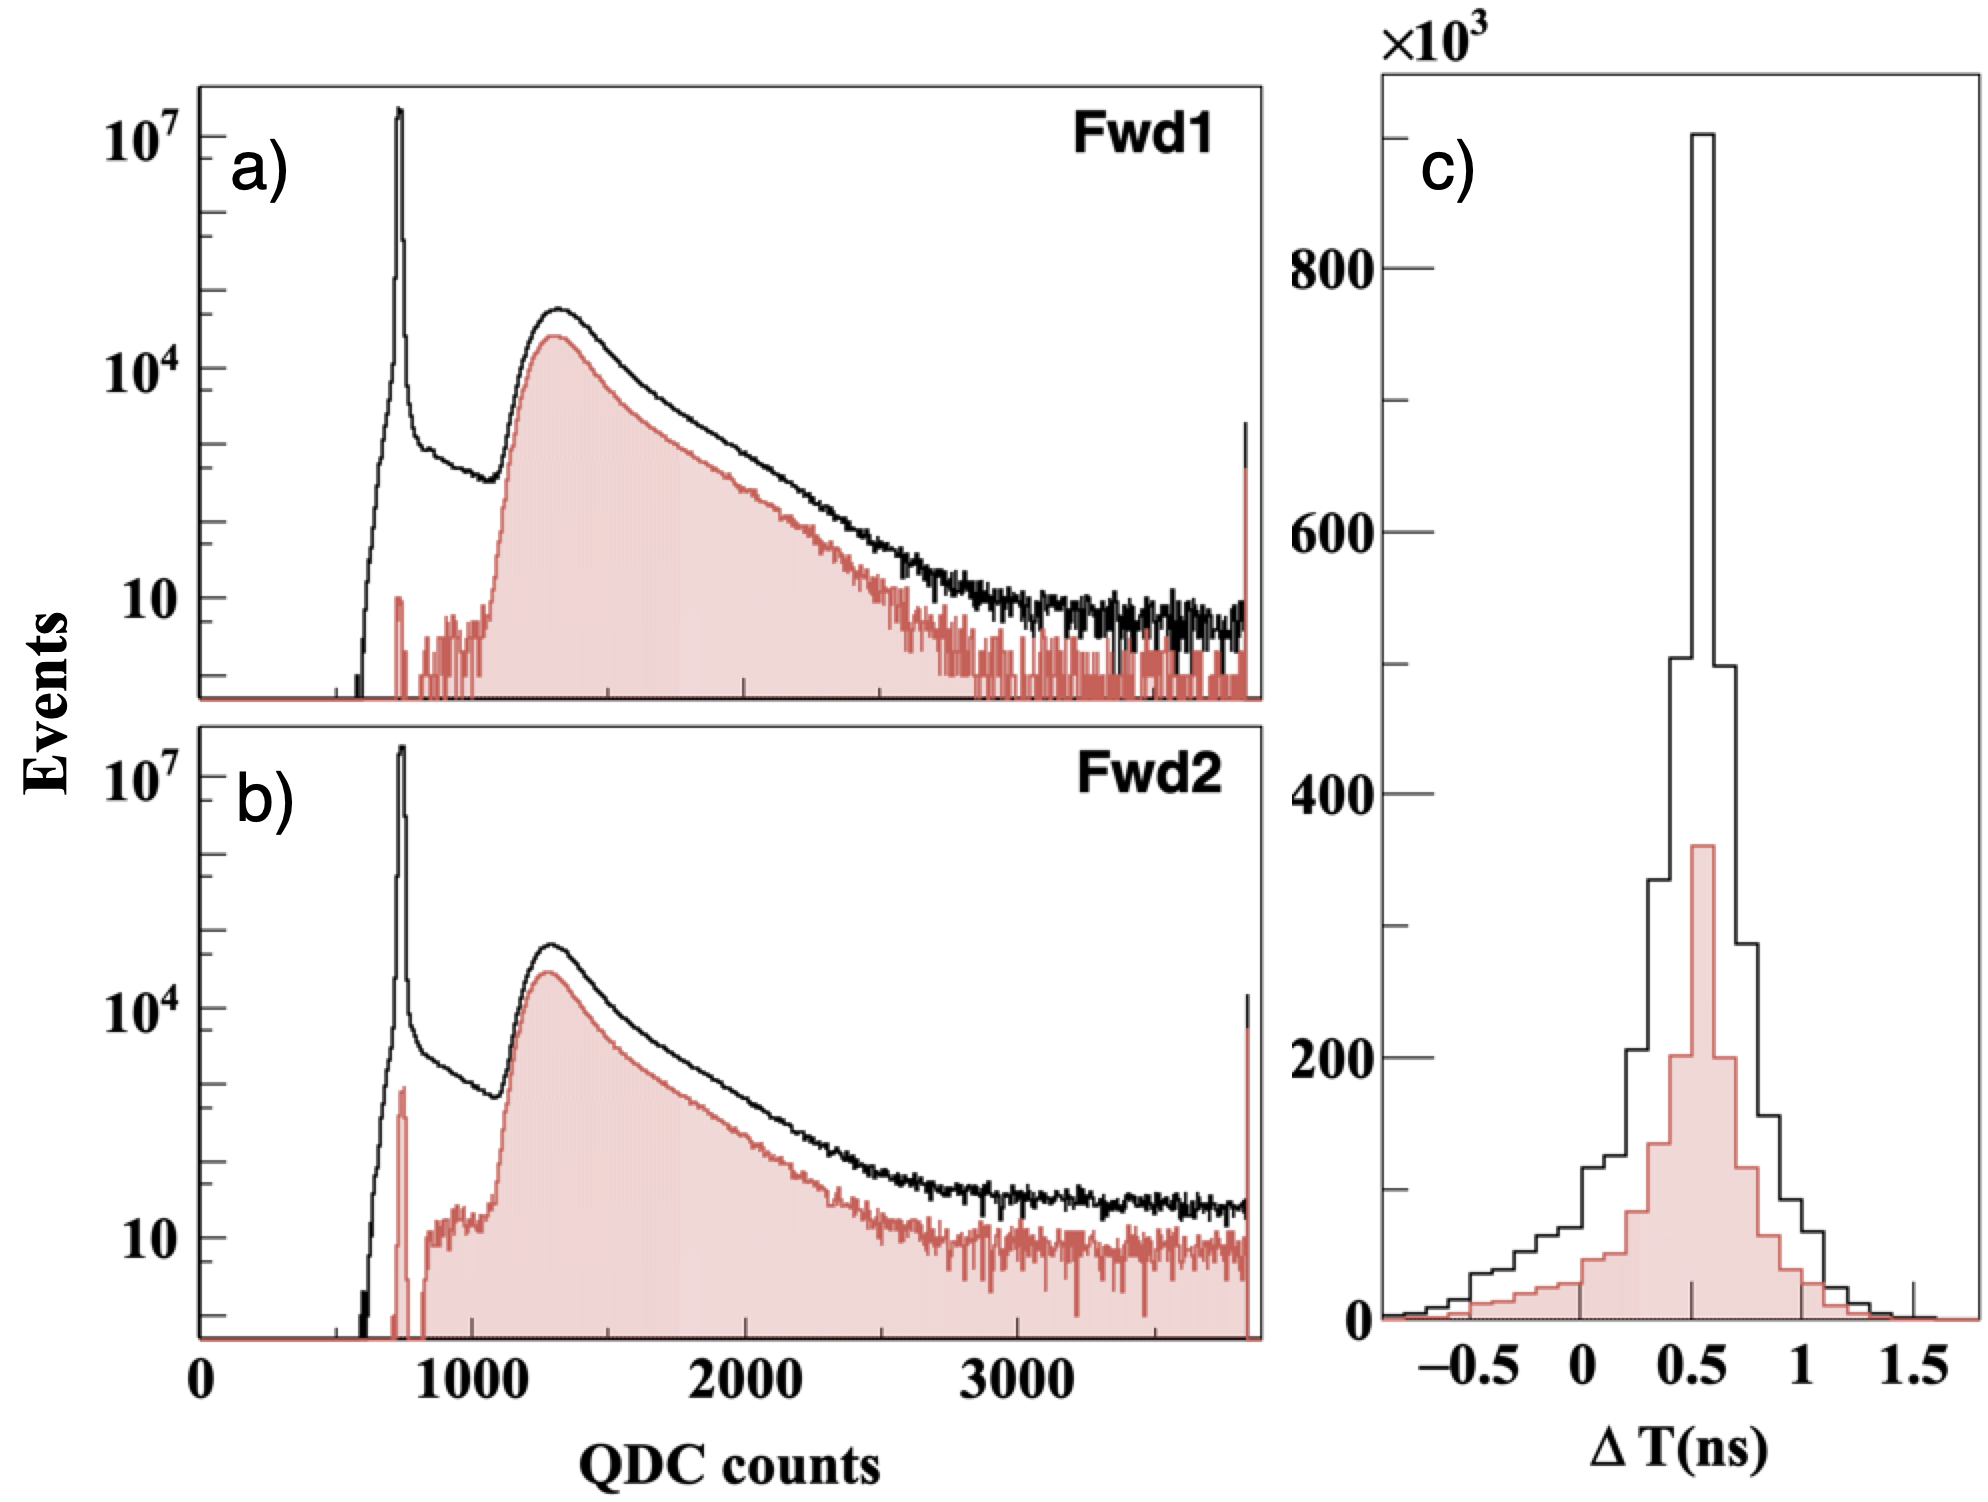
\includegraphics[width=0.45\textwidth]{./fwd_performance_elastic.png}
  \caption{Response of the forward detector: a) the QDC spectrum of the first forward detector module on +X axis;
    b) the QDC spectrum of the second forward detector module on +X axis; c) Time difference between these two modules.
    The black curve are from the events which are triggered by the recoil
    detector.
    The red shading curve are from the elastic scattering event sample.
  }
  \label{fig:fwd_performance}
\end{figure}

The detection efficiencies of the forward modules are also determined with the same elastic scattering sample events, which are about \SI{99.9978}{\percent} and \SI{99.9560}{\percent} respectively.
The scattering effect in the first module causes the slightly worse efficiency in the second layer.
Due to the high efficiency of both modules, the coincidence between them are required to have a
valid hit in the forward detector and the hit time is the average of two modules.

\subsection{Extraction of elastic scattering events at large recoil angles}
\label{sec:recoil_performance}
The typical response of the recoil detector is shown in Fig. \ref{fig:e_map}, in which the energy spectrums of all channels are aggregated together.
The pattern of the recoil energy variation of the elastic scattering with
respect to the channel position is clearly observed.
The elastic peaks lie upon a wide spread of backgrounds which exists over the whole energy range.
At large recoil angles, the elastic peaks are well separated from the high portion of low energy backgrouds.
For these channels, it's possible to extract the elastic peak using a combined fit of the spectrum with an appropriate model of the backgrounds.
% They are well separated from the low energy backgrounds at large recoil angles and are hard to be identified at small recoil angles.
% Thus, different methods are used in the extraction of elastic scattering events
% at large and small recoil angles.
\begin{figure}[htb!]
  \centering
  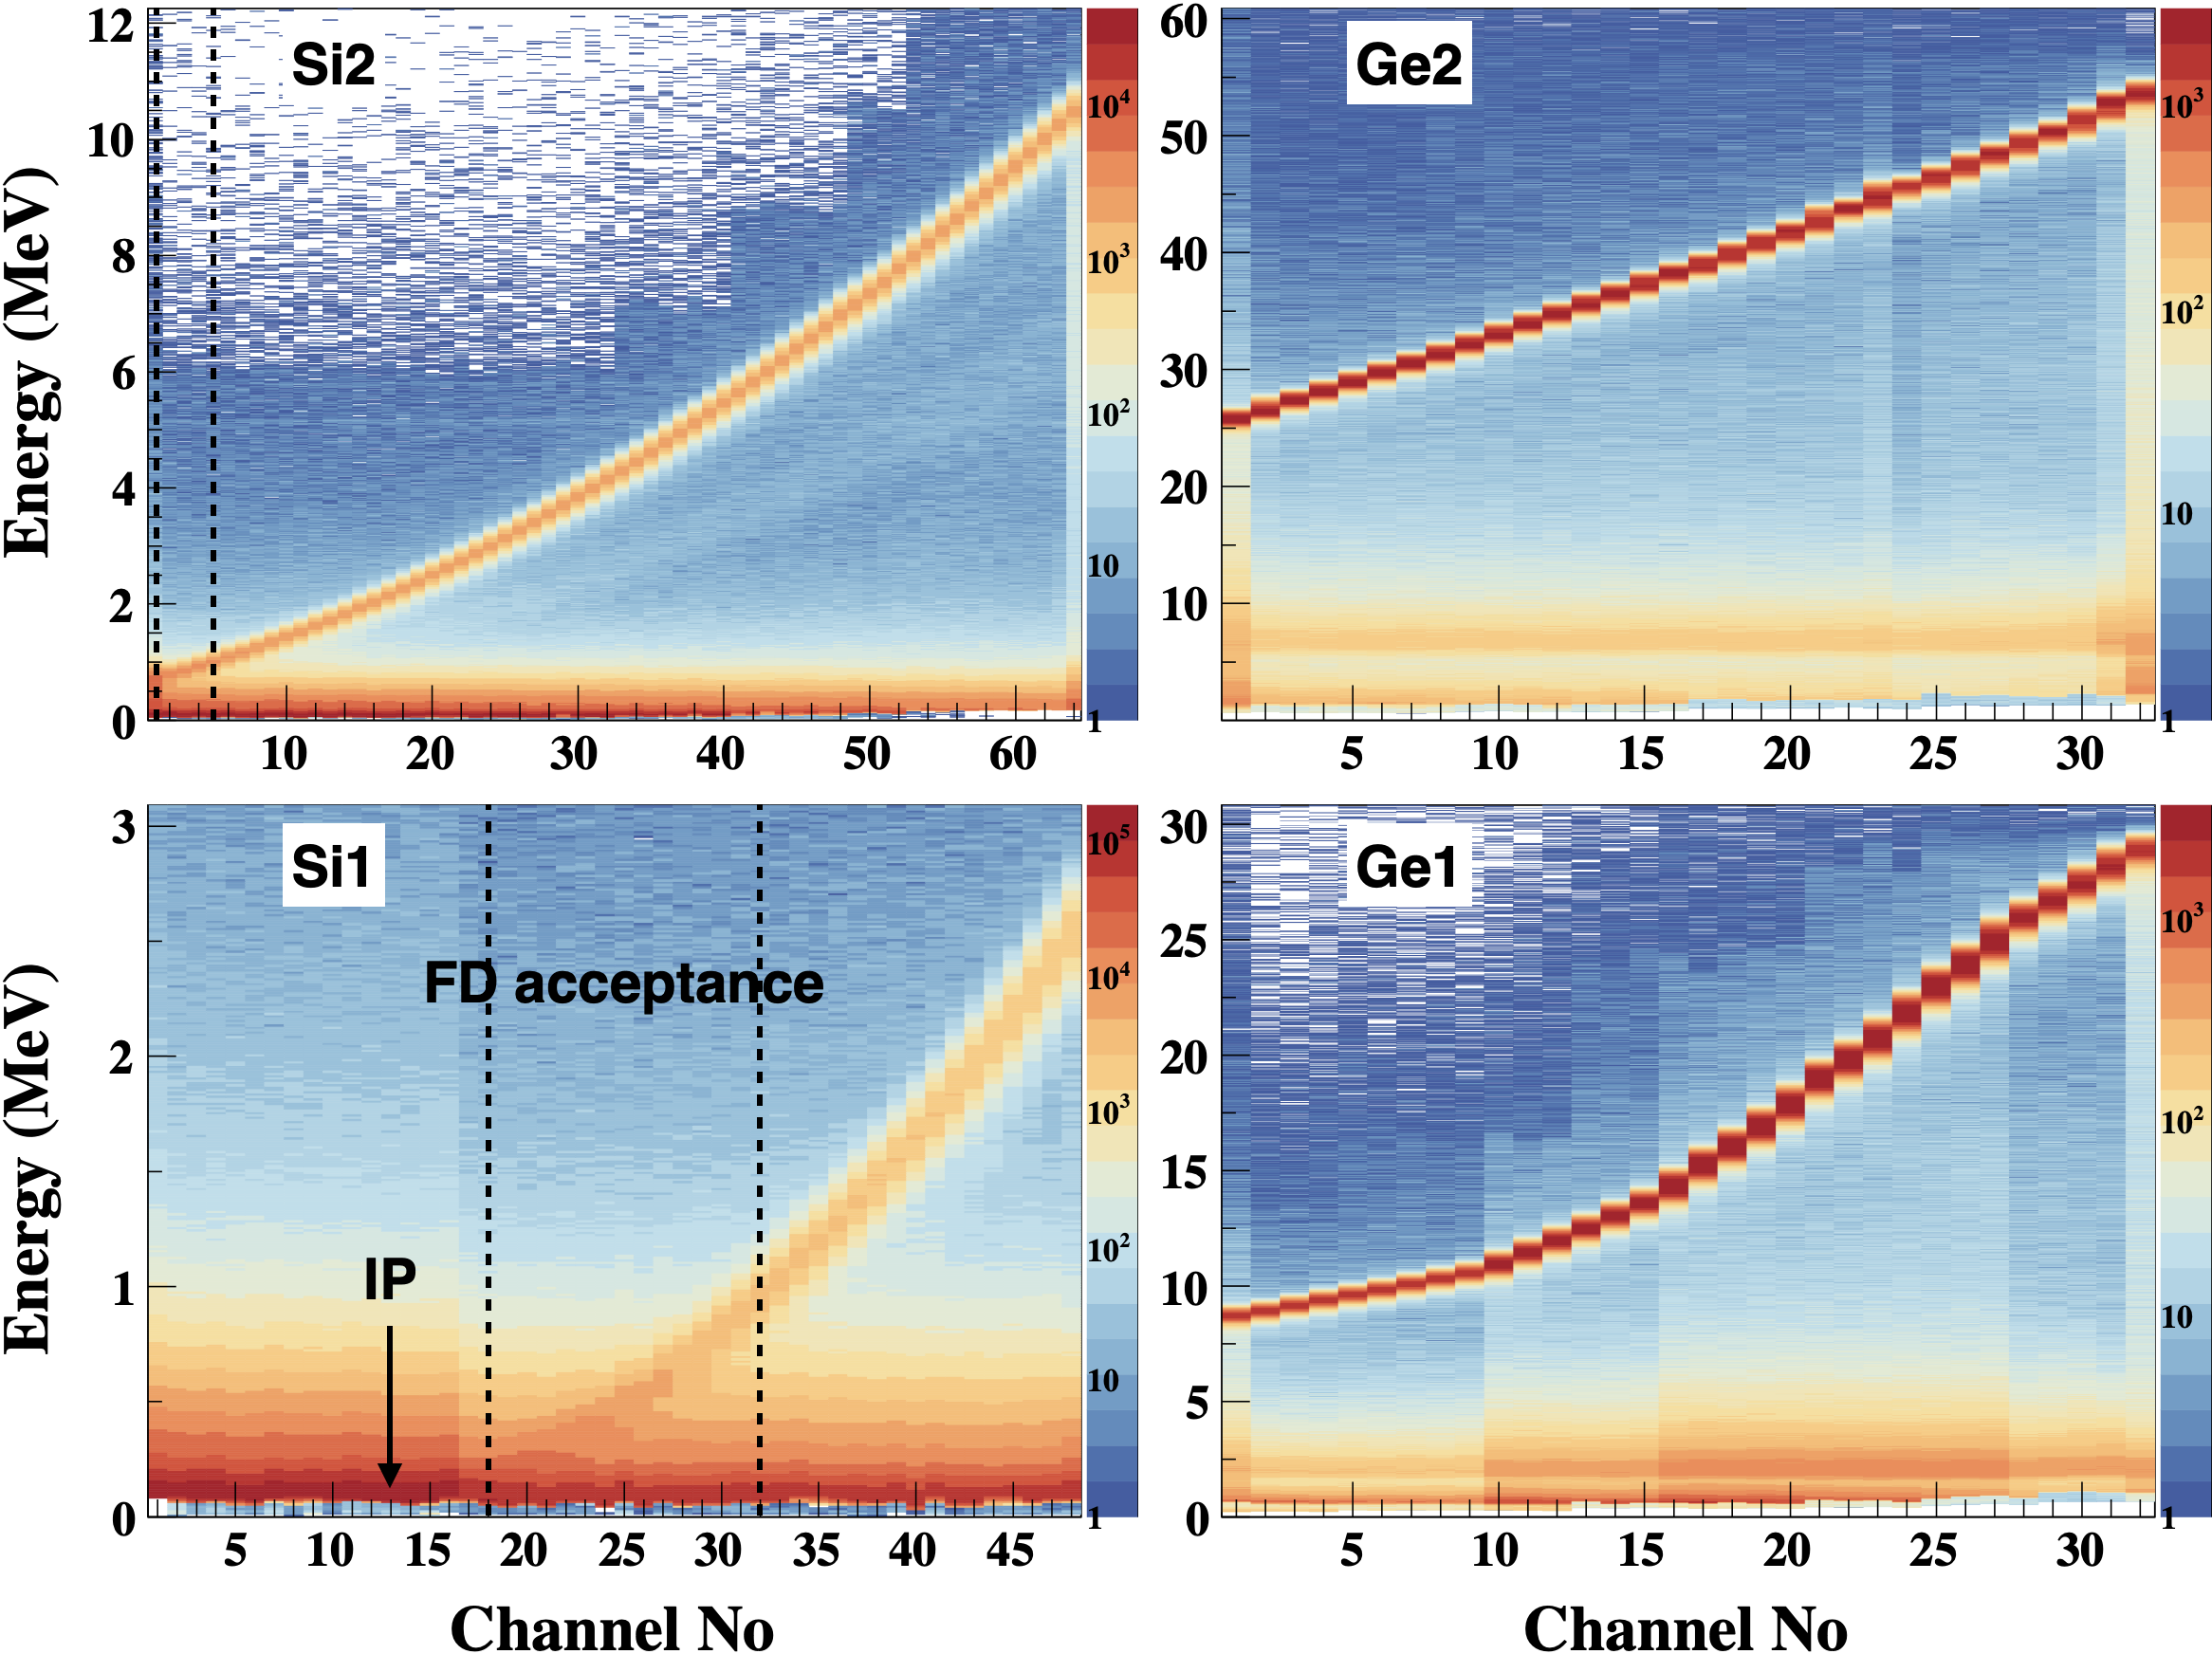
\includegraphics[width=0.48\textwidth]{./e_map.png}
  \caption{Energy spectrums (after clustering) of all channels of the four recoil
    sensors obtained at \SI{2.2}{\momentum}.
    Lower channel number indicates smaller recoil angle.
    IP indicates the channel which is in alignment with
    the beam-target center.
    The group of channels which are fully covered by the forward detector are
    also indicated by the dashed lines on Si1 and Si2.
  }
  \label{fig:e_map}
\end{figure}

An example of the combined fit is shown in Fig. \ref{fig:e_fit}.
Three components are used in the background model: 1) a
fast-decreasing exponetial component which dominates the low energy background; 2)
a slow-decreasing exponetial component which contributes to the high energy
tail; 3) a MIP component which follows the landau distribution.
The MIPs are mainly the pions from the inelastic beam-target interaction, which
have the most probable value of the energy loss of about \num{0.35}, \num{0.35},
\num{2.2}, \SI{7.0}{MeV} in Si1, Si2, Ge1 and Ge2 respectively.
\begin{figure}[h!]
  \centering
  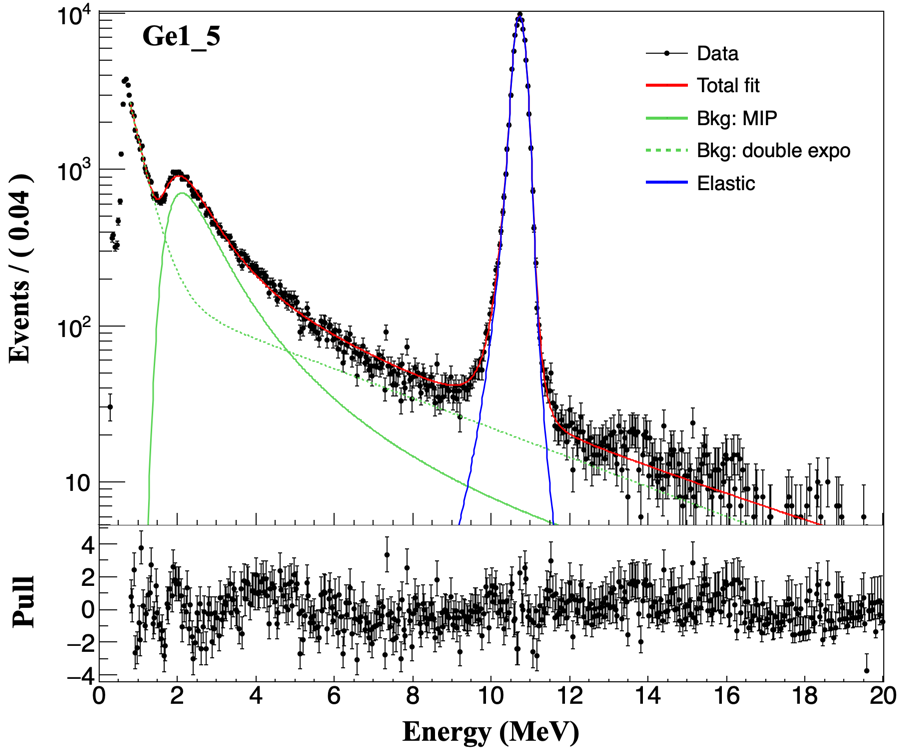
\includegraphics[width=0.45\textwidth]{./e_fit.png}
  \caption{An example of the fit result with background model: MIP + double
    exponential decay.}
  \label{fig:e_fit}
\end{figure}

The fitting model is composed as follows,
\begin{equation}
\begin{aligned}
\mathcal{P}(x) &= N_{1}\lambda_1e^{-\lambda_{1}x}+N_{2}\lambda_2e^{-\lambda_{2}x}\\
&+N_{3}\mathcal{L}(x;\mu_{mip},\sigma_{mip})\ast\mathcal{N}(x;\sigma_{gaus})\\
&+N_{4}\sum_{i=1}^{n_{strips}}{c_{i}f(x;\mu_{i},\sigma_{cb},\alpha_1,n_1,\alpha_2,n_2)}
\end{aligned}
\end{equation}
where the first two items are the exponential components, the third item is the
normalized landau distribution convoluted with the Gaussian response function
and the fourth item is the response function of the recoil detector to the
elastic scattering events from the target.
$N_i (i=1,2,3,4)$ is the event counts for each component of the model.
The double-sided crystal ball function is composed of a Gaussian core and two
power-law tails as follows,
\begin{multline}
  f(x;\mu,\sigma,\alpha_1,n_1,\alpha_2,n_2) = \\
  N\cdot
  \begin{cases}
    \exp(-\frac{(x-\mu)^2}{2\sigma^2}), &\text{for } \alpha_1 < \frac{(x-\mu)}{\sigma} < \alpha_2\\
    A_1(B_1-\frac{x-\mu}{\sigma})^{-n_1}, &\text{for } \frac{(x-\mu)}{\sigma} \leqslant \alpha_1\\
    A_2(B_2+\frac{x-\mu}{\sigma})^{-n_2}, &\text{for } \frac{(x-\mu)}{\sigma} \geqslant \alpha_2
  \end{cases} 
\end{multline}
where
\begin{align}
  A_i &= (\frac{n_i}{\abs{\alpha_i}})^{n_i}\cdot\exp(-\frac{\alpha_i^2}{2}) &,(i=1,2)\\
  B_i &= \frac{n_i}{\abs{\alpha_i}} - \abs{\alpha_i} &,(i=1,2)
\end{align}
The elastic peak is fitted with the double-sided
crystal ball distribution \cite{crystal_ball}, which is composed of a Gaussian core and two
power-law tails at low-end and high-end of the core.
This model of elastic peak describes the response better than the pure Gaussian distribution.
% The two tails can be explained by the small fraction of events which have ambiguity
% of the assignment of hit position because of hitting the gap region between the neighboring strips.

The mean and sigma of the Gaussian core are extracted as the response parameter
of this channel and the area under the fitted elastic peak is extracted as
the count of the elastic scattering events hitting this channel.

\subsection{Extraction of elastic scattering events at small recoil angles}
The accuracy of the extraction method deterioates at smaller recoil angles, because the elastic peak:
1) overlaps with the MIP peak; 2) is supressed by the large amouts of low energy backgrounds.
A pre-selection of the elastic scattering events is needed to improve the extraction.
For the channels which are covered by the forward detector, the correlation
between the recoil proton and the scattering proton is utilized for the selection.

% Elastic selection based on TOF-E
The time-of-flight (TOF) of the recoil proton and its kinetic energy (E)
follows $TOF = l\sqrt{m_p/2E}$, where $l$ is the distance of
the recoil detector to the interaction point, $m_p$ is the proton mass.
Due to the small flight-time variation of the forward scattering proton, TOF of
the recoil proton can be approximated by the difference between the hit time of the recoil detector and the forward detector.
The typical TOF-E spectrum obtained on a single recoil channel is shown in the inner subplot of Fig. \ref{fig:tof-e}. 
\begin{figure}[h!]
  \centering
  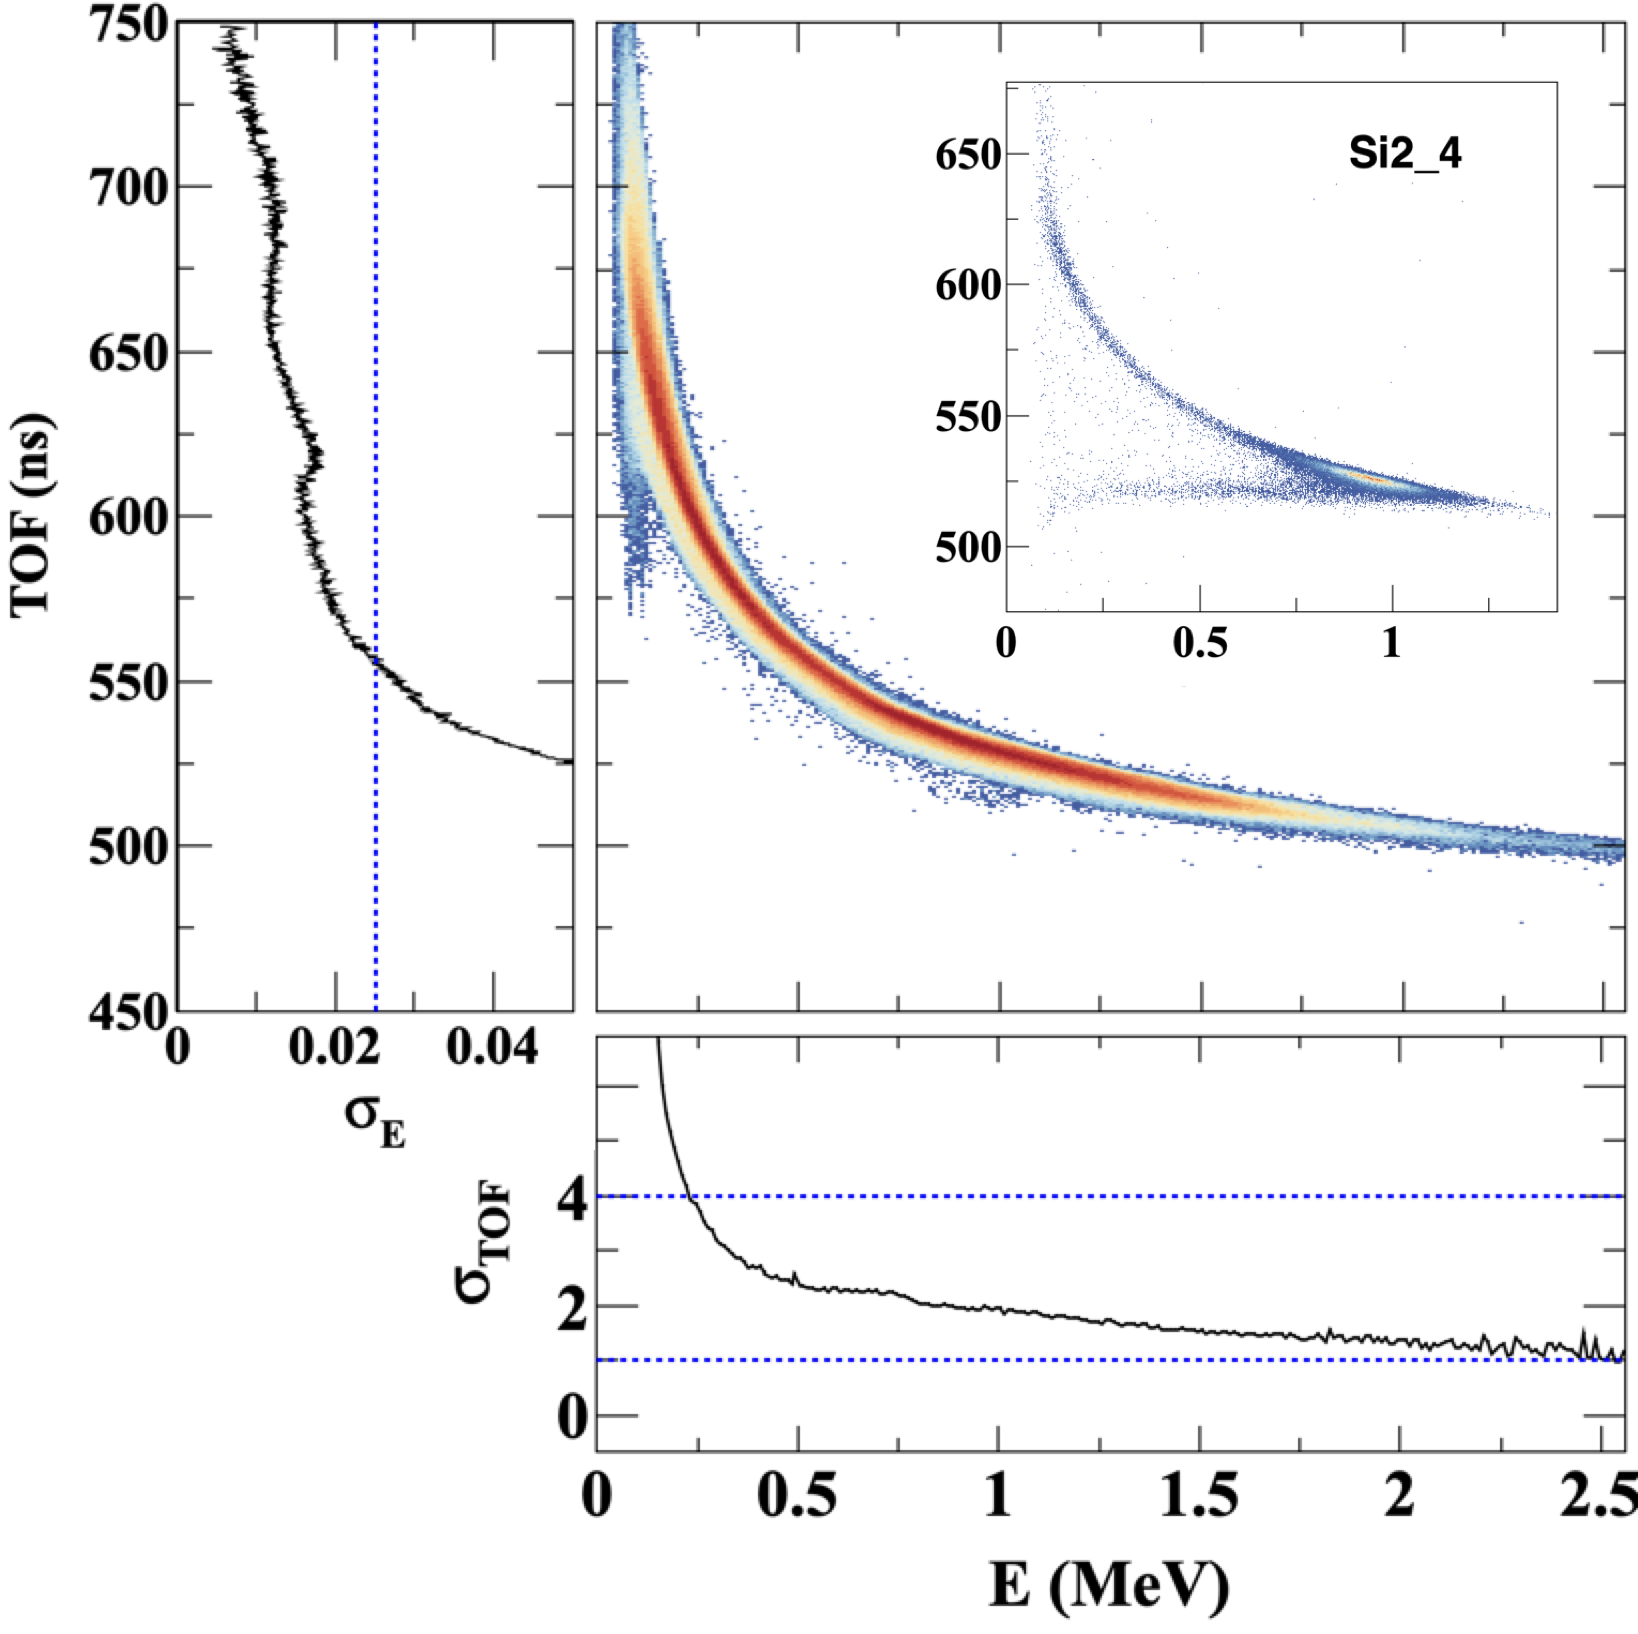
\includegraphics[width=0.45\textwidth]{./tofe_sigma.png}
  \caption{
    TOF-E spectrum of the recoil proton at \SI{2.2}{\momentum}. The data is from all
    strips which are either fully or partly covered by the forward detector.}
  \label{fig:tof-e}
\end{figure}
Three features are recognized in the plot: 1) the wide elastic peak (around
\SI{0.9}{\MeV} in this example);
2) the upper band spreading from the recoil trigger threshold value around
\SI{50}{\keV} to the elastic peak; 3) the horizontal band which splits from the
elastic peak. 
These are common features found in all channels covered by the forward detector.
Since the spectrum has been corrected with the time-walk parameters, the horizontal band matches the time-walk effect.
This band originates from the elastic events hitting the edge of the recoil sensors.
The upper band fullfills the correct TOF-E relation of the recoil proton and it comes
from the residual target gas distribution.

% Selection based on fwd-rec coincidence
Most background events are already supressed by requiring that both
the recoil detector are triggered and the forward detector has a valid
hit from the beam proton, \textit{i.e.}, the QDC amplitudes of both forward detector
are larger than the lower threshold of \num{1000}.
% selection of elastic events and the recoil sigma distribution
More accurate selection of the elastic events is carried out on the TOF-E spectrum as follows:
1) the central region of the upper band and the elastic peak is cut out;
2) the profile of the central region is performed on a \SI{10}{\keV} step to get an
estimate of the TOF-E relation and the standard deviation $\sigma_{TOF}$ at each energy step.
3) the obtained TOF-E relation combining with the $[-5\sigma_{TOF}, 5\sigma_{TOF}]$ window is finally applied to filter out the elastic events.
This selection effectively filter out all the full elastic events, \textit{i.e.}
elastic events in which the recoil proton deposit all its energy in the recoil
sensor and the scattered proton penetrating through the forward detector. 
An aggregate of the selected events from all channels of the recoil detector are
shown in \ref{fig:tof-e}, with the two side plots showing the variation of the
standard deviation ($\sigma_{TOF}$ and $\sigma_{E}$) of the profile along the E-axis and TOF-axis respectively.
The deteoriation of the resolution near the edge of the spectrum is mainly
contributed by the extremely large or small derivative of the TOF-E curve at
these energy values.
The modest value of $\sigma_{TOF}$ and $\sigma_{E}$ is about
\SI{2.5}{\nano\second} and \SI{25}{\keV} respectively.

% combined fit using coulomb background and coverage of the fwd acceptance
\begin{figure}[h!]
  \centering
  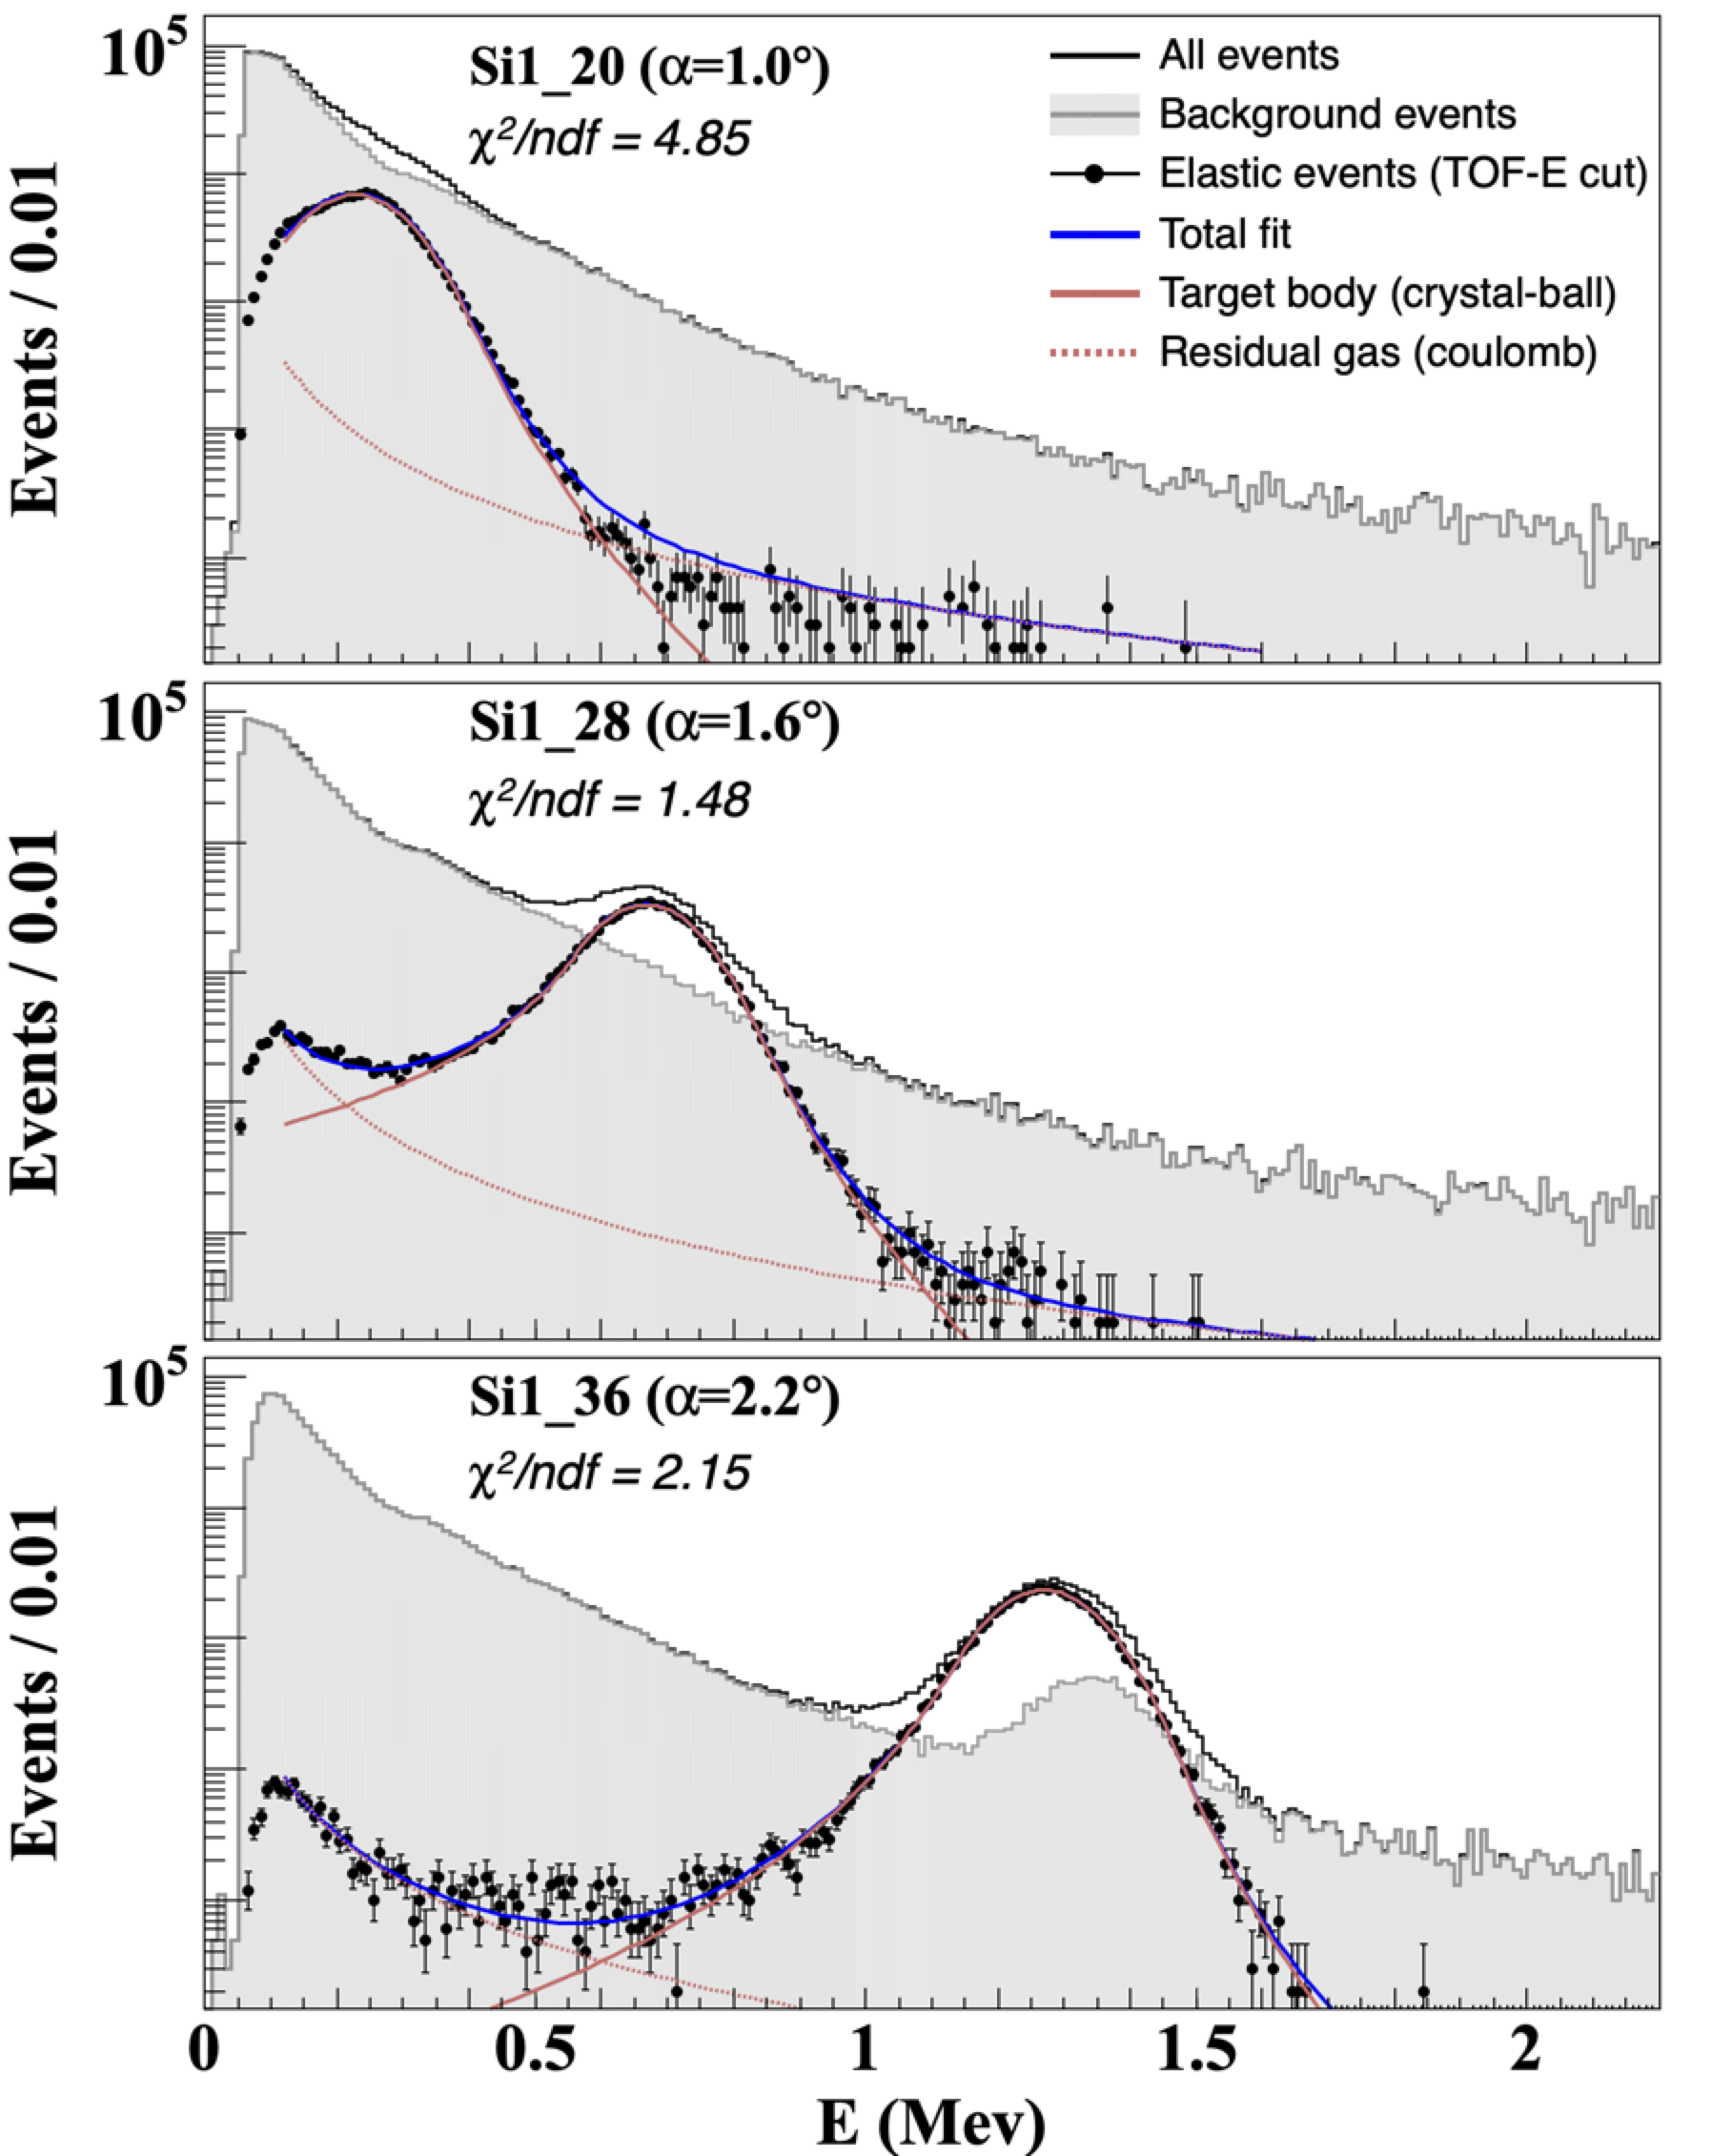
\includegraphics[width=0.45\textwidth]{./tofe_cut_comparison.png}
  \caption{Energy spectrums (black) of two channels at small recoil angle on Si1 (from
    \SI{2.2}{\momentum} data). The elastic peak (red) overlaps with the low-energy background
    spectrum (grey) and is hardly recognizable in the original spectrum. These low-energy background events are effectively surpressed by applying the TOF-E relation selection.}
  \label{fig:cut}
\end{figure}


\subsection{Minimum measurable $|t|$}
\label{minimum_t}

Fig. \ref{fig:measured_vs_calculated} shows the comparison between the measured
energy of the elastic peak and the expected energy of the recoil proton from elastic scattering at \SI{2.2}{\momentum}.
A limit is observed around \SI{200}{\keV}, which corresponds to $|t| \approx  \SI{0.0004}{\tmom}$.
Same analysis on other three beam momentums shows that the minimum measurable
recoil energies are all below \SI{300}{\keV}, which is well beblow the desired $|t|_{min}$.

\begin{figure}[h!]
  \centering
  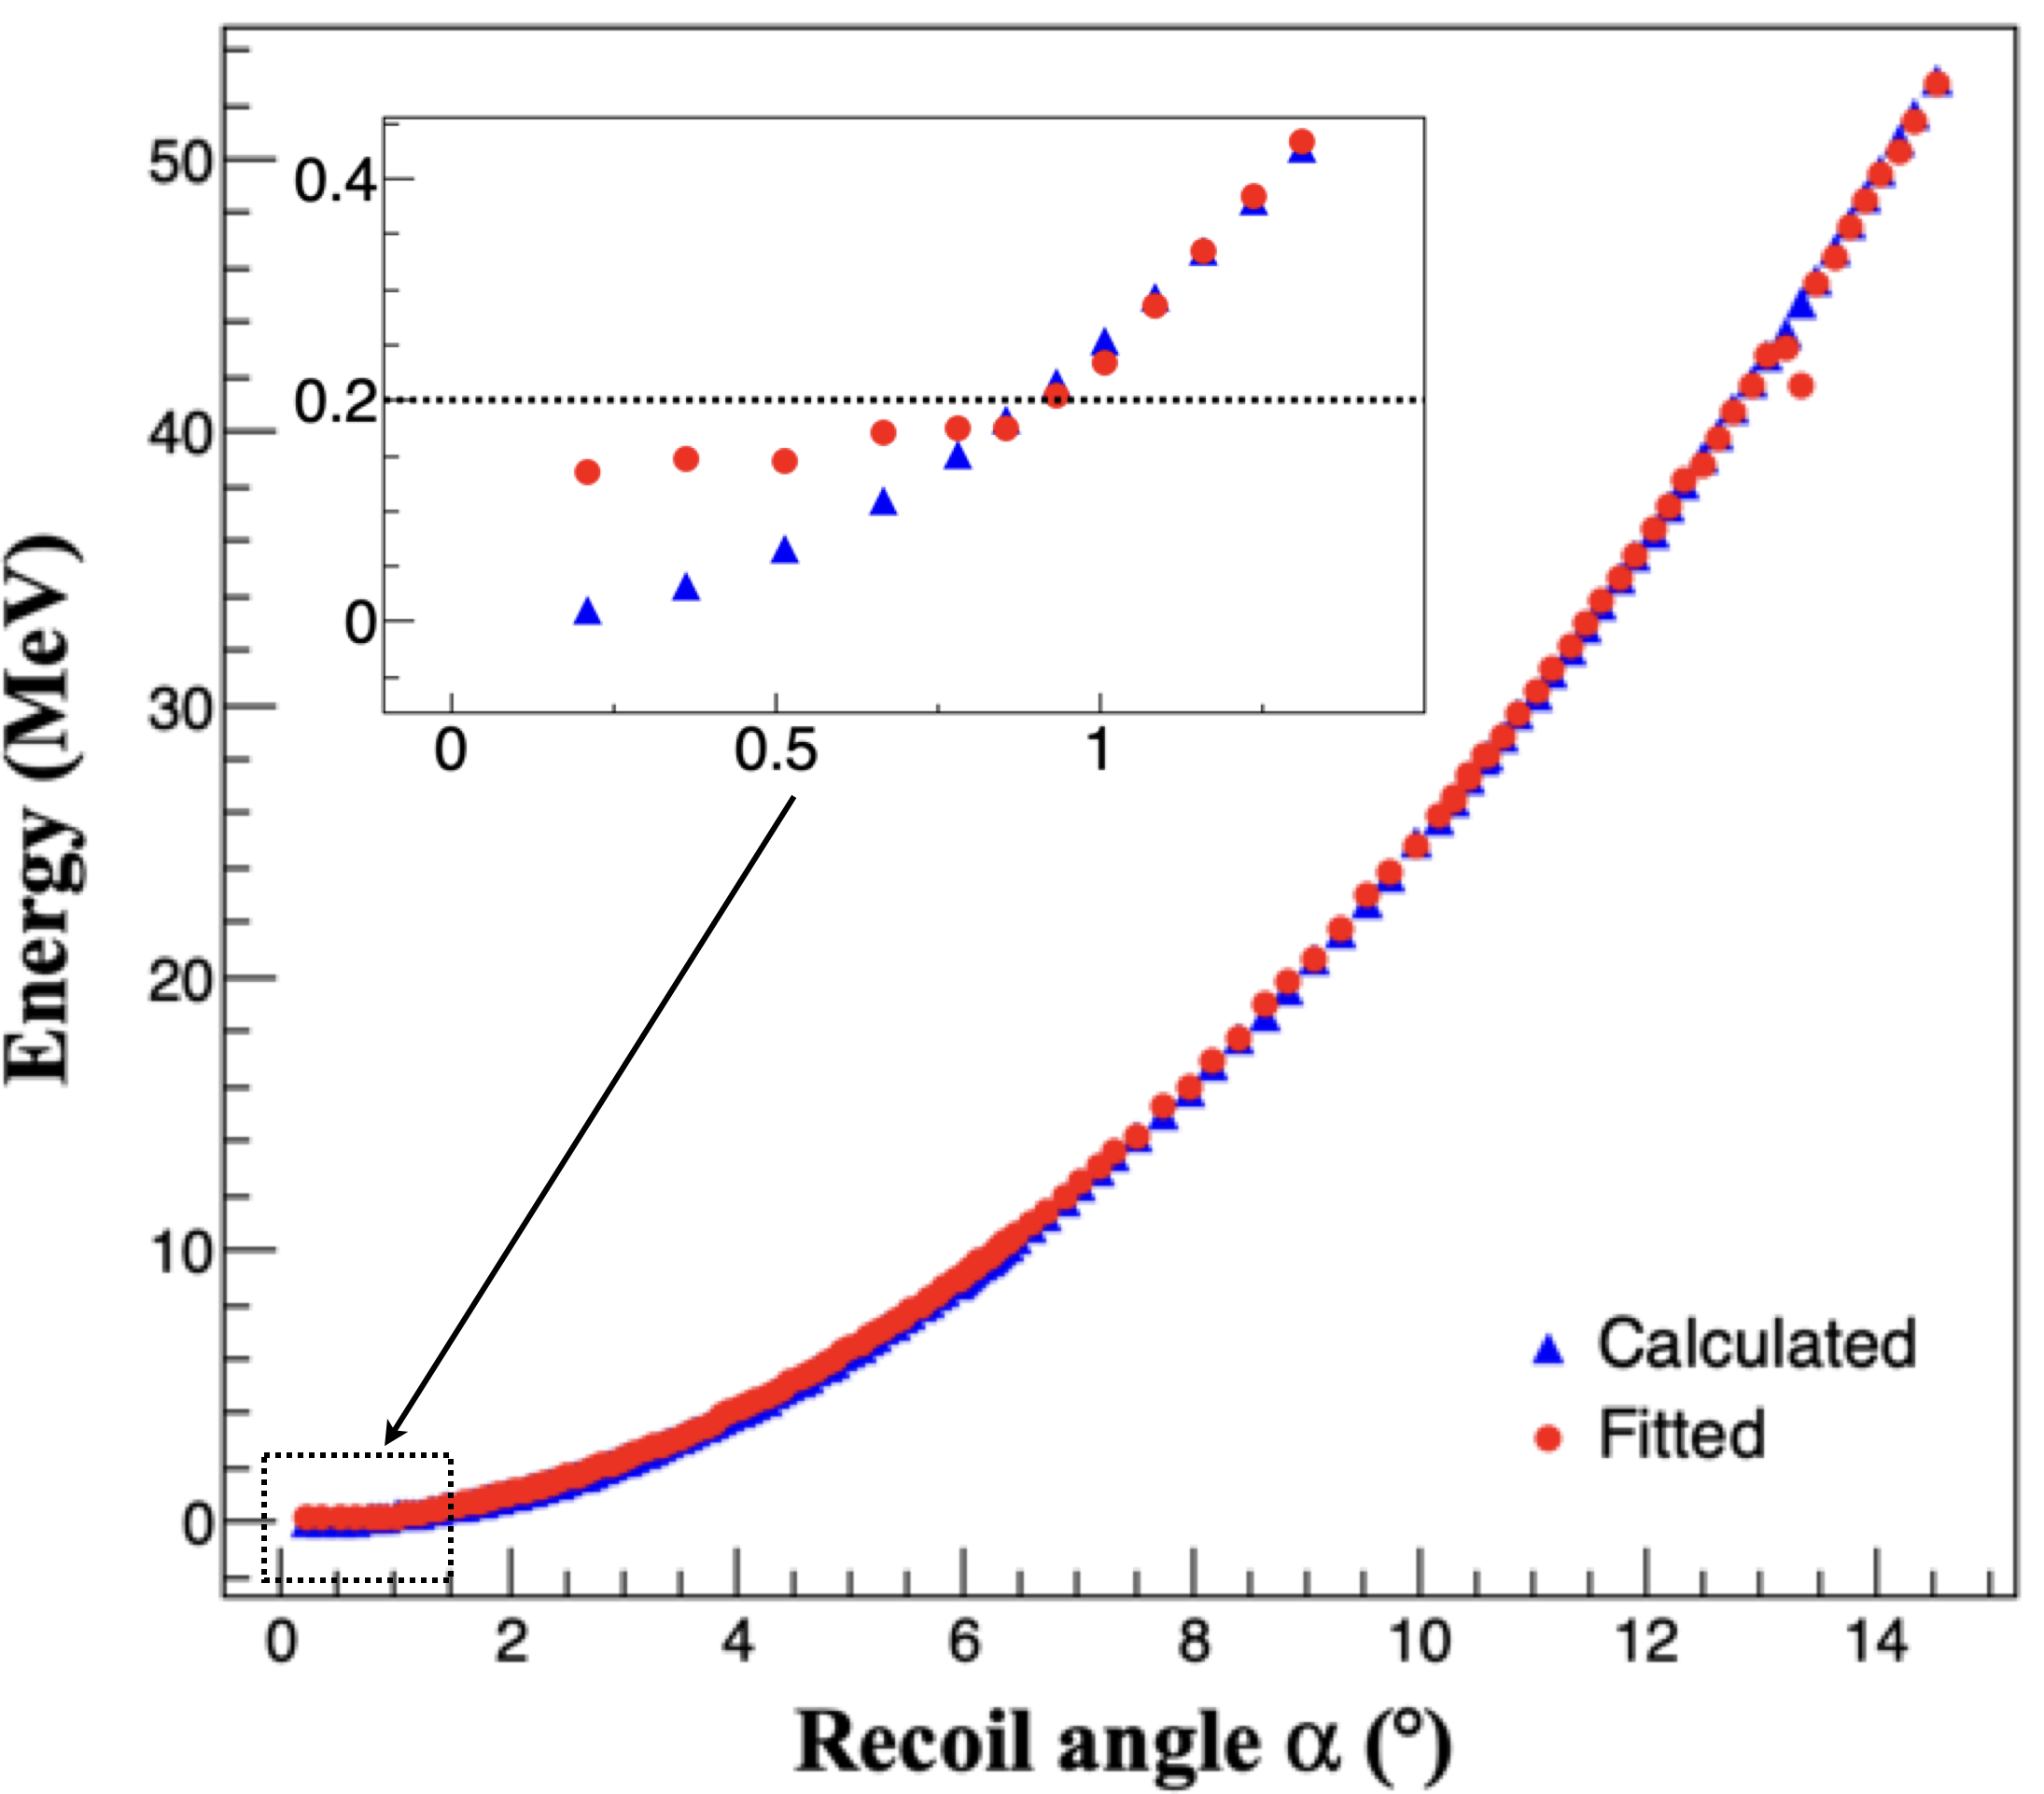
\includegraphics[width=0.42\textwidth]{./calc_vs_measured_2.2_angle_combined.png}
  \caption{
    Comparison of measured (red circle) and calculated (blue triangle) recoil energy with respect to the strip position along z-axis (i.e. beam direction) at beam momentum \SI{2.2}{\momentum}.}
  \label{fig:measured_vs_calculated}
\end{figure}


\section{Conclusion and Outlook}
\label{sec:conclusion}

The commissioning of the full KOALA setup at COSY, specifically of the new forward detector, is successful.
A strong correlation between the recoil detector and the forward detector is
observed for the covered region of the forward detector.
The idea of using the TOF-E relation of the recoil proton to extract elastic
scattering events is verified.
Preliminary analysis shows that lower |t| beyond the design requirement of \SI{0.0008}{\tmom} can be reached from \SIrange{2.2}{3.0}{\momentum}. 

However, it's also found that the forward detector could not cover the full
length of strips at larger recoil angles within the designed acceptance.
% that even in the forward-covered region, some elastic
% events do not generate coincidence between the recoil and forward detector.
This is mainly due to the fact that the stochastic cooling is not stable all the time
and the beam profile is larger than expected.
More strict requirement for the stochastic cooling is needed for future experiments.
Besides, scintillators with larger size, especially larger width, are also proposed.

The updated DAQ operated in stable condition in the commissioning tests.
But it's found that the limited performance of DAQ will bring an efficiency bias in different
sub-detectors due to the differenct noise triggering level.
Optimization of the DAQ is needed to minimize this bias.
The mask gate in the trigger logic is proposed to be removed in the future.
Thus, more tests of the timestamp-based synchronization in the offline analysis are needed.

\bibliographystyle{elsarticle-num}
\bibliography{reference}

\end{document}
